\documentclass[]{article}
\usepackage{lmodern}
\usepackage{amssymb,amsmath}
\usepackage{ifxetex,ifluatex}
\usepackage{fixltx2e} % provides \textsubscript
\ifnum 0\ifxetex 1\fi\ifluatex 1\fi=0 % if pdftex
  \usepackage[T1]{fontenc}
  \usepackage[utf8]{inputenc}
\else % if luatex or xelatex
  \ifxetex
    \usepackage{mathspec}
  \else
    \usepackage{fontspec}
  \fi
  \defaultfontfeatures{Ligatures=TeX,Scale=MatchLowercase}
\fi
% use upquote if available, for straight quotes in verbatim environments
\IfFileExists{upquote.sty}{\usepackage{upquote}}{}
% use microtype if available
\IfFileExists{microtype.sty}{%
\usepackage{microtype}
\UseMicrotypeSet[protrusion]{basicmath} % disable protrusion for tt fonts
}{}
\usepackage[margin=1in]{geometry}
\usepackage{hyperref}
\hypersetup{unicode=true,
            pdfborder={0 0 0},
            breaklinks=true}
\urlstyle{same}  % don't use monospace font for urls
\usepackage{color}
\usepackage{fancyvrb}
\newcommand{\VerbBar}{|}
\newcommand{\VERB}{\Verb[commandchars=\\\{\}]}
\DefineVerbatimEnvironment{Highlighting}{Verbatim}{commandchars=\\\{\}}
% Add ',fontsize=\small' for more characters per line
\usepackage{framed}
\definecolor{shadecolor}{RGB}{248,248,248}
\newenvironment{Shaded}{\begin{snugshade}}{\end{snugshade}}
\newcommand{\KeywordTok}[1]{\textcolor[rgb]{0.13,0.29,0.53}{\textbf{#1}}}
\newcommand{\DataTypeTok}[1]{\textcolor[rgb]{0.13,0.29,0.53}{#1}}
\newcommand{\DecValTok}[1]{\textcolor[rgb]{0.00,0.00,0.81}{#1}}
\newcommand{\BaseNTok}[1]{\textcolor[rgb]{0.00,0.00,0.81}{#1}}
\newcommand{\FloatTok}[1]{\textcolor[rgb]{0.00,0.00,0.81}{#1}}
\newcommand{\ConstantTok}[1]{\textcolor[rgb]{0.00,0.00,0.00}{#1}}
\newcommand{\CharTok}[1]{\textcolor[rgb]{0.31,0.60,0.02}{#1}}
\newcommand{\SpecialCharTok}[1]{\textcolor[rgb]{0.00,0.00,0.00}{#1}}
\newcommand{\StringTok}[1]{\textcolor[rgb]{0.31,0.60,0.02}{#1}}
\newcommand{\VerbatimStringTok}[1]{\textcolor[rgb]{0.31,0.60,0.02}{#1}}
\newcommand{\SpecialStringTok}[1]{\textcolor[rgb]{0.31,0.60,0.02}{#1}}
\newcommand{\ImportTok}[1]{#1}
\newcommand{\CommentTok}[1]{\textcolor[rgb]{0.56,0.35,0.01}{\textit{#1}}}
\newcommand{\DocumentationTok}[1]{\textcolor[rgb]{0.56,0.35,0.01}{\textbf{\textit{#1}}}}
\newcommand{\AnnotationTok}[1]{\textcolor[rgb]{0.56,0.35,0.01}{\textbf{\textit{#1}}}}
\newcommand{\CommentVarTok}[1]{\textcolor[rgb]{0.56,0.35,0.01}{\textbf{\textit{#1}}}}
\newcommand{\OtherTok}[1]{\textcolor[rgb]{0.56,0.35,0.01}{#1}}
\newcommand{\FunctionTok}[1]{\textcolor[rgb]{0.00,0.00,0.00}{#1}}
\newcommand{\VariableTok}[1]{\textcolor[rgb]{0.00,0.00,0.00}{#1}}
\newcommand{\ControlFlowTok}[1]{\textcolor[rgb]{0.13,0.29,0.53}{\textbf{#1}}}
\newcommand{\OperatorTok}[1]{\textcolor[rgb]{0.81,0.36,0.00}{\textbf{#1}}}
\newcommand{\BuiltInTok}[1]{#1}
\newcommand{\ExtensionTok}[1]{#1}
\newcommand{\PreprocessorTok}[1]{\textcolor[rgb]{0.56,0.35,0.01}{\textit{#1}}}
\newcommand{\AttributeTok}[1]{\textcolor[rgb]{0.77,0.63,0.00}{#1}}
\newcommand{\RegionMarkerTok}[1]{#1}
\newcommand{\InformationTok}[1]{\textcolor[rgb]{0.56,0.35,0.01}{\textbf{\textit{#1}}}}
\newcommand{\WarningTok}[1]{\textcolor[rgb]{0.56,0.35,0.01}{\textbf{\textit{#1}}}}
\newcommand{\AlertTok}[1]{\textcolor[rgb]{0.94,0.16,0.16}{#1}}
\newcommand{\ErrorTok}[1]{\textcolor[rgb]{0.64,0.00,0.00}{\textbf{#1}}}
\newcommand{\NormalTok}[1]{#1}
\usepackage{graphicx,grffile}
\makeatletter
\def\maxwidth{\ifdim\Gin@nat@width>\linewidth\linewidth\else\Gin@nat@width\fi}
\def\maxheight{\ifdim\Gin@nat@height>\textheight\textheight\else\Gin@nat@height\fi}
\makeatother
% Scale images if necessary, so that they will not overflow the page
% margins by default, and it is still possible to overwrite the defaults
% using explicit options in \includegraphics[width, height, ...]{}
\setkeys{Gin}{width=\maxwidth,height=\maxheight,keepaspectratio}
\IfFileExists{parskip.sty}{%
\usepackage{parskip}
}{% else
\setlength{\parindent}{0pt}
\setlength{\parskip}{6pt plus 2pt minus 1pt}
}
\setlength{\emergencystretch}{3em}  % prevent overfull lines
\providecommand{\tightlist}{%
  \setlength{\itemsep}{0pt}\setlength{\parskip}{0pt}}
\setcounter{secnumdepth}{0}
% Redefines (sub)paragraphs to behave more like sections
\ifx\paragraph\undefined\else
\let\oldparagraph\paragraph
\renewcommand{\paragraph}[1]{\oldparagraph{#1}\mbox{}}
\fi
\ifx\subparagraph\undefined\else
\let\oldsubparagraph\subparagraph
\renewcommand{\subparagraph}[1]{\oldsubparagraph{#1}\mbox{}}
\fi

%%% Use protect on footnotes to avoid problems with footnotes in titles
\let\rmarkdownfootnote\footnote%
\def\footnote{\protect\rmarkdownfootnote}

%%% Change title format to be more compact
\usepackage{titling}

% Create subtitle command for use in maketitle
\newcommand{\subtitle}[1]{
  \posttitle{
    \begin{center}\large#1\end{center}
    }
}

\setlength{\droptitle}{-2em}

  \title{}
    \pretitle{\vspace{\droptitle}}
  \posttitle{}
    \author{}
    \preauthor{}\postauthor{}
    \date{}
    \predate{}\postdate{}
  
\usepackage{booktabs}
\usepackage{longtable}
\usepackage{array}
\usepackage{multirow}
\usepackage[table]{xcolor}
\usepackage{wrapfig}
\usepackage{float}
\usepackage{colortbl}
\usepackage{pdflscape}
\usepackage{tabu}
\usepackage{threeparttable}
\usepackage{threeparttablex}
\usepackage[normalem]{ulem}
\usepackage{makecell}

\begin{document}

\begin{Shaded}
\begin{Highlighting}[]
\KeywordTok{library}\NormalTok{(here)}
\end{Highlighting}
\end{Shaded}

\begin{verbatim}
## here() starts at /Users/henrikeckermann/workspace/research_master/minor_research_project/article/analyses/bibo
\end{verbatim}

\begin{Shaded}
\begin{Highlighting}[]
\KeywordTok{library}\NormalTok{(ggplot2)}
\KeywordTok{library}\NormalTok{(tidyverse)}
\end{Highlighting}
\end{Shaded}

\begin{verbatim}
## -- Attaching packages ----------------------------------------------------------------------------------------- tidyverse 1.2.1 --
\end{verbatim}

\begin{verbatim}
## v tibble  1.4.2     v purrr   0.2.5
## v tidyr   0.8.2     v dplyr   0.7.8
## v readr   1.3.1     v stringr 1.3.1
## v tibble  1.4.2     v forcats 0.3.0
\end{verbatim}

\begin{verbatim}
## -- Conflicts -------------------------------------------------------------------------------------------- tidyverse_conflicts() --
## x dplyr::filter() masks stats::filter()
## x dplyr::lag()    masks stats::lag()
\end{verbatim}

\begin{Shaded}
\begin{Highlighting}[]
\KeywordTok{library}\NormalTok{(papaja)}
\KeywordTok{library}\NormalTok{(ggpubr)}
\end{Highlighting}
\end{Shaded}

\begin{verbatim}
## Loading required package: magrittr
\end{verbatim}

\begin{verbatim}
## 
## Attaching package: 'magrittr'
\end{verbatim}

\begin{verbatim}
## The following object is masked from 'package:purrr':
## 
##     set_names
\end{verbatim}

\begin{verbatim}
## The following object is masked from 'package:tidyr':
## 
##     extract
\end{verbatim}

\begin{Shaded}
\begin{Highlighting}[]
\KeywordTok{library}\NormalTok{(microbiome)}
\end{Highlighting}
\end{Shaded}

\begin{verbatim}
## Loading required package: phyloseq
\end{verbatim}

\begin{verbatim}
## 
## microbiome R package (microbiome.github.com)
##     
## 
## 
##  Copyright (C) 2011-2018 Leo Lahti et al. <microbiome.github.io>
\end{verbatim}

\begin{verbatim}
## 
## Attaching package: 'microbiome'
\end{verbatim}

\begin{verbatim}
## The following object is masked from 'package:base':
## 
##     transform
\end{verbatim}

\begin{Shaded}
\begin{Highlighting}[]
\KeywordTok{source}\NormalTok{(}\StringTok{"https://raw.githubusercontent.com/HenrikEckermann/in_use/master/reporting.R"}\NormalTok{)}
\end{Highlighting}
\end{Shaded}

\begin{verbatim}
## 
## Attaching package: 'glue'
\end{verbatim}

\begin{verbatim}
## The following object is masked from 'package:dplyr':
## 
##     collapse
\end{verbatim}

\begin{Shaded}
\begin{Highlighting}[]
\KeywordTok{load}\NormalTok{(}\KeywordTok{here}\NormalTok{(}\StringTok{"data/cc_analyses_workspace.RData"}\NormalTok{))}
\end{Highlighting}
\end{Shaded}

\section{3. Results}\label{results}

\subsection{3.1. Microbiota composition}\label{microbiota-composition}

Thirteen genus like groups from the \emph{Actinobacteria},
\emph{Firmicutes}, \emph{Proteobacteria} and phyla showed an average
abundance of \(\gt 0.05\)\% in at least 20\% of the samples (Figure 1).
Overall the microbiota was dominated by \emph{Bifidobacterium} with an
average abundance of more than 50\%. Followed by facultative anaerobic
\emph{Bacilli} (\emph{Streptococcus spp}, \emph{Enterococcus},
\emph{Lactobacilllus} and \emph{Granulicatella}). The general variation
of relative abundance of all taxa was quite high, with
\emph{Bifidobacterium} for instance ranging from 0.2\% to 89\%.

Figure 2 shows microbiota composition (Aitchison distance) for the first
four principal components within the CC (A) and within the noCC (B)
group. The starting point of the arrow indicate the microbiota
composition at T0, whereas the endpoint corresponds the composition at
T1. The plots do not reveal a systematic shift due to CC attendance over
time. Instead, microbiota composition development between time points
appears to be highly individual.

\begin{Shaded}
\begin{Highlighting}[]
\KeywordTok{ggarrange}\NormalTok{(}
\NormalTok{    biplot_cc[[}\DecValTok{1}\NormalTok{]] }\OperatorTok{+}\StringTok{ }\KeywordTok{xlim}\NormalTok{(}\OperatorTok{-}\FloatTok{12.5}\NormalTok{, }\DecValTok{5}\NormalTok{) }\OperatorTok{+}\StringTok{ }\KeywordTok{ggtitle}\NormalTok{(}\StringTok{'A'}\NormalTok{), }
\NormalTok{    biplot_cc[[}\DecValTok{2}\NormalTok{]] }\OperatorTok{+}\StringTok{ }\KeywordTok{xlim}\NormalTok{(}\OperatorTok{-}\FloatTok{12.5}\NormalTok{, }\DecValTok{5}\NormalTok{) }\OperatorTok{+}\StringTok{ }\KeywordTok{ggtitle}\NormalTok{(}\StringTok{'B'}\NormalTok{), }
\NormalTok{    biplot_cc[[}\DecValTok{3}\NormalTok{]] }\OperatorTok{+}\StringTok{ }\KeywordTok{xlim}\NormalTok{(}\OperatorTok{-}\FloatTok{12.5}\NormalTok{, }\DecValTok{5}\NormalTok{) }\OperatorTok{+}\StringTok{ }\KeywordTok{ggtitle}\NormalTok{(}\StringTok{'C'}\NormalTok{), }
\NormalTok{    biplot_cc[[}\DecValTok{4}\NormalTok{]] }\OperatorTok{+}\StringTok{ }\KeywordTok{xlim}\NormalTok{(}\OperatorTok{-}\FloatTok{12.5}\NormalTok{, }\DecValTok{5}\NormalTok{) }\OperatorTok{+}\StringTok{ }\KeywordTok{ggtitle}\NormalTok{(}\StringTok{'D'}\NormalTok{), }
    \DataTypeTok{nrow =} \DecValTok{2}\NormalTok{, }\DataTypeTok{ncol =} \DecValTok{2}\NormalTok{, }
    \DataTypeTok{common.legend =}\NormalTok{ T)}
\end{Highlighting}
\end{Shaded}

\begin{verbatim}
## Scale for 'x' is already present. Adding another scale for 'x', which
## will replace the existing scale.
## Scale for 'x' is already present. Adding another scale for 'x', which
## will replace the existing scale.
## Scale for 'x' is already present. Adding another scale for 'x', which
## will replace the existing scale.
## Scale for 'x' is already present. Adding another scale for 'x', which
## will replace the existing scale.
\end{verbatim}

\begin{figure}
\centering
\includegraphics{results_files/figure-latex/unnamed-chunk-2-1.pdf}
\caption{Development of microbiota composition over time within CC (A
and C) and no CC (B and D).}
\end{figure}

\begin{Shaded}
\begin{Highlighting}[]
\KeywordTok{ggarrange}\NormalTok{(}
\NormalTok{    biplot_time[[}\DecValTok{1}\NormalTok{]] }\OperatorTok{+}\StringTok{ }\KeywordTok{xlim}\NormalTok{(}\OperatorTok{-}\FloatTok{12.5}\NormalTok{, }\DecValTok{5}\NormalTok{) }\OperatorTok{+}\StringTok{ }\KeywordTok{ggtitle}\NormalTok{(}\StringTok{'A'}\NormalTok{), }
\NormalTok{    biplot_time[[}\DecValTok{2}\NormalTok{]] }\OperatorTok{+}\StringTok{ }\KeywordTok{xlim}\NormalTok{(}\OperatorTok{-}\FloatTok{12.5}\NormalTok{, }\DecValTok{5}\NormalTok{) }\OperatorTok{+}\StringTok{ }\KeywordTok{ggtitle}\NormalTok{(}\StringTok{'B'}\NormalTok{), }
\NormalTok{    biplot_time[[}\DecValTok{3}\NormalTok{]] }\OperatorTok{+}\StringTok{ }\KeywordTok{xlim}\NormalTok{(}\OperatorTok{-}\FloatTok{12.5}\NormalTok{, }\DecValTok{5}\NormalTok{) }\OperatorTok{+}\StringTok{ }\KeywordTok{ggtitle}\NormalTok{(}\StringTok{'C'}\NormalTok{), }
\NormalTok{    biplot_time[[}\DecValTok{4}\NormalTok{]] }\OperatorTok{+}\StringTok{ }\KeywordTok{xlim}\NormalTok{(}\OperatorTok{-}\FloatTok{12.5}\NormalTok{, }\DecValTok{5}\NormalTok{) }\OperatorTok{+}\StringTok{ }\KeywordTok{ggtitle}\NormalTok{(}\StringTok{'D'}\NormalTok{), }
    \DataTypeTok{nrow =} \DecValTok{2}\NormalTok{, }\DataTypeTok{ncol =} \DecValTok{2}\NormalTok{, }
    \DataTypeTok{common.legend =}\NormalTok{ T)}
\end{Highlighting}
\end{Shaded}

\begin{verbatim}
## Scale for 'x' is already present. Adding another scale for 'x', which
## will replace the existing scale.
## Scale for 'x' is already present. Adding another scale for 'x', which
## will replace the existing scale.
## Scale for 'x' is already present. Adding another scale for 'x', which
## will replace the existing scale.
## Scale for 'x' is already present. Adding another scale for 'x', which
## will replace the existing scale.
\end{verbatim}

\begin{figure}
\centering
\includegraphics{results_files/figure-latex/unnamed-chunk-2-2.pdf}
\caption{Development of microbiota composition over time within CC (A
and C) and no CC (B and D).}
\end{figure}

\begin{Shaded}
\begin{Highlighting}[]
\NormalTok{biplot_time_}\DecValTok{2}\NormalTok{ <-}\StringTok{ }\KeywordTok{biplot}\NormalTok{(pseq.clr, }\DataTypeTok{facet =} \StringTok{"cc"}\NormalTok{, }\DataTypeTok{connect_series =} \StringTok{"time"}\NormalTok{)}
\end{Highlighting}
\end{Shaded}

\begin{verbatim}
## Warning in class(x) <- c(subclass, "tbl_df", "tbl", "data.frame"): Setting
## class(x) to multiple strings ("tbl_df", "tbl", ...); result will no longer
## be an S4 object
\end{verbatim}

\begin{Shaded}
\begin{Highlighting}[]
\KeywordTok{ggarrange}\NormalTok{(biplot_time_}\DecValTok{2}\NormalTok{[[}\DecValTok{1}\NormalTok{]], biplot_time_}\DecValTok{2}\NormalTok{[[}\DecValTok{1}\NormalTok{]], }\DataTypeTok{nrow =} \DecValTok{2}\NormalTok{)}
\end{Highlighting}
\end{Shaded}

\begin{figure}
\centering
\includegraphics{results_files/figure-latex/unnamed-chunk-2-3.pdf}
\caption{Development of microbiota composition over time within CC (A
and C) and no CC (B and D).}
\end{figure}

\begin{Shaded}
\begin{Highlighting}[]
\NormalTok{otus.clr }\OperatorTok\StringTok{ }\KeywordTok{column_to_rownames}\NormalTok{(}\StringTok{"sample_id"}\NormalTok{) }\OperatorTok
\StringTok{  }\KeywordTok{t}\NormalTok{() }\OperatorTok\StringTok{ }\KeywordTok{as.data.frame}\NormalTok{() }\OperatorTok\StringTok{ }\KeywordTok{summarise_all}\NormalTok{(sum)}
\end{Highlighting}
\end{Shaded}

\begin{verbatim}
##       sa_10000      sa_10038     sa_10118      sa_10211     sa_10230
## 1 2.131628e-14 -5.329071e-15 3.730349e-14 -1.199041e-14 7.105427e-15
##        sa_10247       sa_1025     sa_10268       sa_1028      sa_1030
## 1 -3.375078e-14 -3.019807e-14 -2.04281e-14 -4.973799e-14 4.440892e-16
##         sa_1045      sa_1054      sa_10657      sa_10742    sa_10747
## 1 -7.549517e-15 1.465494e-14 -1.554312e-14 -7.105427e-15 5.77316e-15
##         sa_108     sa_10812     sa_10840     sa_10944      sa_11040
## 1 1.776357e-14 3.907985e-14 5.373479e-14 7.549517e-15 -3.019807e-14
##       sa_11136     sa_11180     sa_11183      sa_11190      sa_11210
## 1 1.865175e-14 2.753353e-14 3.019807e-14 -1.110223e-14 -4.174439e-14
##         sa_1127      sa_11392     sa_11488      sa_11498        sa_115
## 1 -7.105427e-15 -5.151435e-14 2.220446e-14 -3.996803e-14 -5.595524e-14
##       sa_11517     sa_11615      sa_11628      sa_1164      sa_11659
## 1 1.865175e-14 7.105427e-15 -8.881784e-15 3.108624e-14 -5.684342e-14
##         sa_1294         sa_13       sa_1389       sa_1559      sa_1577
## 1 -4.884981e-14 -5.329071e-15 -5.151435e-14 -4.440892e-16 5.506706e-14
##         sa_1659      sa_1678      sa_1743       sa_1857     sa_1866
## 1 -2.975398e-14 2.131628e-14 1.199041e-14 -2.664535e-14 1.24345e-14
##        sa_1939       sa_1972      sa_1999      sa_2052      sa_2116
## 1 2.797762e-14 -1.909584e-14 1.021405e-14 7.993606e-15 4.707346e-14
##        sa_2124      sa_2298      sa_2337       sa_2384       sa_2424
## 1 8.437695e-15 4.796163e-14 7.993606e-15 -3.108624e-15 -2.442491e-14
##        sa_2431      sa_2495      sa_2511       sa_2541      sa_2691
## 1 5.595524e-14 5.062617e-14 1.776357e-14 -3.197442e-14 1.509903e-14
##        sa_2717      sa_2826      sa_2864       sa_2908       sa_2952
## 1 1.776357e-15 9.769963e-15 3.419487e-14 -4.440892e-14 -3.774758e-14
##        sa_3146      sa_3212       sa_3232      sa_3238       sa_3407
## 1 2.309264e-14 1.776357e-14 -6.217249e-15 7.105427e-15 -2.842171e-14
##        sa_3434       sa_3535      sa_3548      sa_3573        sa_358
## 1 8.881784e-15 -1.731948e-14 8.881784e-16 4.796163e-14 -5.373479e-14
##         sa_3634       sa_372       sa_3758       sa_3791       sa_3833
## 1 -2.176037e-14 4.618528e-14 -1.421085e-14 -5.018208e-14 -5.506706e-14
##        sa_3873      sa_3887       sa_3892       sa_3935       sa_3947
## 1 4.440892e-15 4.796163e-14 -2.131628e-14 -2.664535e-15 -9.325873e-15
##         sa_4003        sa_426       sa_433       sa_438       sa_4416
## 1 -2.575717e-14 -2.087219e-14 2.398082e-14 2.131628e-14 -5.373479e-14
##         sa_4478       sa_4511       sa_4574       sa_4630      sa_4779
## 1 -3.907985e-14 -2.664535e-14 -1.154632e-14 -4.263256e-14 1.776357e-14
##         sa_4941       sa_4966      sa_4990       sa_5002      sa_5045
## 1 -3.730349e-14 -3.019807e-14 5.684342e-14 -5.595524e-14 -2.88658e-14
##        sa_5073       sa_5131      sa_5288       sa_5374       sa_5450
## 1 5.551115e-14 -2.220446e-14 4.396483e-14 -1.776357e-15 -4.973799e-14
##         sa_5453      sa_5469        sa_549       sa_5512      sa_553
## 1 -2.176037e-14 5.506706e-14 -4.218847e-14 -4.973799e-14 2.04281e-14
##        sa_5551       sa_5637      sa_5725      sa_5740      sa_5780
## 1 9.325873e-15 -1.154632e-14 1.021405e-14 3.508305e-14 3.463896e-14
##        sa_5818      sa_5861      sa_5864      sa_5875       sa_5906
## 1 5.417888e-14 1.332268e-14 -3.68594e-14 4.796163e-14 -4.485301e-14
##         sa_5928       sa_5986      sa_6067      sa_6195      sa_6223
## 1 -4.396483e-14 -1.598721e-14 1.421085e-14 1.065814e-14 5.062617e-14
##        sa_6328       sa_6332      sa_6369      sa_6380       sa_6430
## 1 2.975398e-14 -3.197442e-14 5.506706e-14 4.707346e-14 -5.595524e-14
##         sa_6648      sa_6661       sa_6743       sa_6773      sa_6852
## 1 -1.776357e-15 2.930989e-14 -3.730349e-14 -4.218847e-14 3.996803e-14
##         sa_6976       sa_6989      sa_7040      sa_7116     sa_7134
## 1 -3.552714e-14 -1.509903e-14 7.105427e-15 -1.64313e-14 3.28626e-14
##        sa_7161      sa_7166       sa_7168      sa_7198        sa_726
## 1 1.332268e-14 3.064216e-14 -4.440892e-16 3.552714e-15 -5.151435e-14
##        sa_7322      sa_7340      sa_7341       sa_740      sa_7417
## 1 1.909584e-14 2.753353e-14 5.728751e-14 2.531308e-14 1.509903e-14
##         sa_7422       sa_7451      sa_7459       sa_7477       sa_7538
## 1 -4.796163e-14 -4.707346e-14 4.884981e-14 -1.865175e-14 -2.309264e-14
##        sa_7599      sa_7679       sa_7759 sa_7768      sa_7778
## 1 3.108624e-14 4.840572e-14 -4.352074e-14       0 1.065814e-14
##        sa_7972       sa_8026       sa_8061       sa_832     sa_8342
## 1 3.419487e-14 -3.108624e-15 -1.154632e-14 2.398082e-14 1.24345e-14
##       sa_8657       sa_8678       sa_8703      sa_8715        sa_881
## 1 3.28626e-14 -2.575717e-14 -9.325873e-15 1.332268e-14 -2.930989e-14
##         sa_8818       sa_8833      sa_8856       sa_886      sa_8869
## 1 -5.151435e-14 -3.463896e-14 1.820766e-14 3.952394e-14 2.664535e-14
##       sa_8998       sa_9001       sa_9022       sa_9030 sa_9080
## 1 1.24345e-14 -4.796163e-14 -2.753353e-14 -1.731948e-14       0
##         sa_9091      sa_9232      sa_9343       sa_9352      sa_9408
## 1 -1.776357e-14 3.730349e-14 6.217249e-15 -4.440892e-14 2.220446e-14
##        sa_9412      sa_9462        sa_953      sa_9543      sa_9691
## 1 1.776357e-15 2.975398e-14 -2.309264e-14 4.396483e-14 2.531308e-14
##        sa_987      sa_9913      sa_9924       sa_9951       sa_9953
## 1 4.52971e-14 5.329071e-15 3.996803e-14 -4.396483e-14 -5.684342e-14
##         sa_9994
## 1 -5.329071e-15
\end{verbatim}

\subsection{3.2 Permutational multivariate
ANOVA}\label{permutational-multivariate-anova}

We performed PERMANOVA for 10 imputed datasets (see methods), which all
yield similar results. We compared the overall community composition
using PERMANOVA based on Aitchison distance metric. An assumption for
PERMANOVA is multivariate homogeneity of group dispersions (variances)
{[}@Anderson2017{]}. We used the function \emph{betadisper}
{[}@vegan2017{]}, which utilizes the \emph{PERMDISP2} procedure as
implemented by Marti Anderson and found that this assumption was met for
the factors \emph{childcare} \emph{F}(1,194) = 0.19, \emph{p} = .188,
\emph{time} \emph{F}(1,194) = 1.73, \emph{p} = .190 and the subgroups
that result out of the interaction of \emph{time} and \emph{cc}
\emph{F}(3,192) = 1.19, \emph{p} = .313. According to PERMANOVA,
breastfeeding and age significantly predicted overall community
composition (see table x). Figure 5 shows the genera that mostly changed
as a function of each predictor. There is no significant effect of CC
over time on overall community composition.

\begin{Shaded}
\begin{Highlighting}[]
\KeywordTok{apa_table}\NormalTok{(pm_table)}
\end{Highlighting}
\end{Shaded}

\begin{verbatim}
## 
## 
## \begin{table}[tbp]
## \begin{center}
## \begin{threeparttable}
## \caption{\label{tab:unnamed-chunk-4}}
## \begin{tabular}{lllllll}
## \toprule
## Model Parameter & \multicolumn{1}{c}{Sum of Squares} & \multicolumn{1}{c}{Mean Sum of Squares} & \multicolumn{1}{c}{F} & \multicolumn{1}{c}{Df} & \multicolumn{1}{c}{p} & \multicolumn{1}{c}{R Square}\\
## \midrule
## time & 58.44 & 58.444 & 1.469 & 1.00 & 0.12 & 0.01\\
## cc & 52.64 & 52.636 & 1.323 & 1.00 & 0.181 & 0.01\\
## age\_d\_s & 79.55 & 79.553 & 2 & 1.00 & 0.026 & 0.01\\
## bf\_count\_s & 197.06 & 197.06 & 4.954 & 1.00 & 0.001 & 0.02\\
## time:cc & 36.23 & 36.229 & 0.911 & 1.00 & 0.505 & 0.00\\
## Residuals & 7,558.55 & 39.782 & - & 190.00 & - & 0.95\\
## Total & 7,982.47 & - & - & 195.00 & - & 1.00\\
## \bottomrule
## \end{tabular}
## \end{threeparttable}
## \end{center}
## \end{table}
\end{verbatim}

\begin{Shaded}
\begin{Highlighting}[]
\KeywordTok{ggarrange}\NormalTok{(}
\NormalTok{    pmps[[}\DecValTok{1}\NormalTok{]] }\OperatorTok{+}\StringTok{ }\KeywordTok{ggtitle}\NormalTok{(}\StringTok{'A'}\NormalTok{), }
\NormalTok{    pmps[[}\DecValTok{2}\NormalTok{]] }\OperatorTok{+}\StringTok{ }\KeywordTok{ggtitle}\NormalTok{(}\StringTok{'B'}\NormalTok{), }
\NormalTok{    pmps[[}\DecValTok{3}\NormalTok{]] }\OperatorTok{+}\StringTok{ }\KeywordTok{ggtitle}\NormalTok{(}\StringTok{'C'}\NormalTok{), }
\NormalTok{    pmps[[}\DecValTok{4}\NormalTok{]] }\OperatorTok{+}\StringTok{ }\KeywordTok{ggtitle}\NormalTok{(}\StringTok{'D'}\NormalTok{), }
\NormalTok{    pmps[[}\DecValTok{5}\NormalTok{]] }\OperatorTok{+}\StringTok{ }\KeywordTok{ggtitle}\NormalTok{(}\StringTok{'E'}\NormalTok{),}
    \DataTypeTok{nrow =} \DecValTok{3}\NormalTok{, }\DataTypeTok{ncol =} \DecValTok{2}\NormalTok{, }\DataTypeTok{common.legend =}\NormalTok{ T)}
\end{Highlighting}
\end{Shaded}

\begin{figure}
\centering
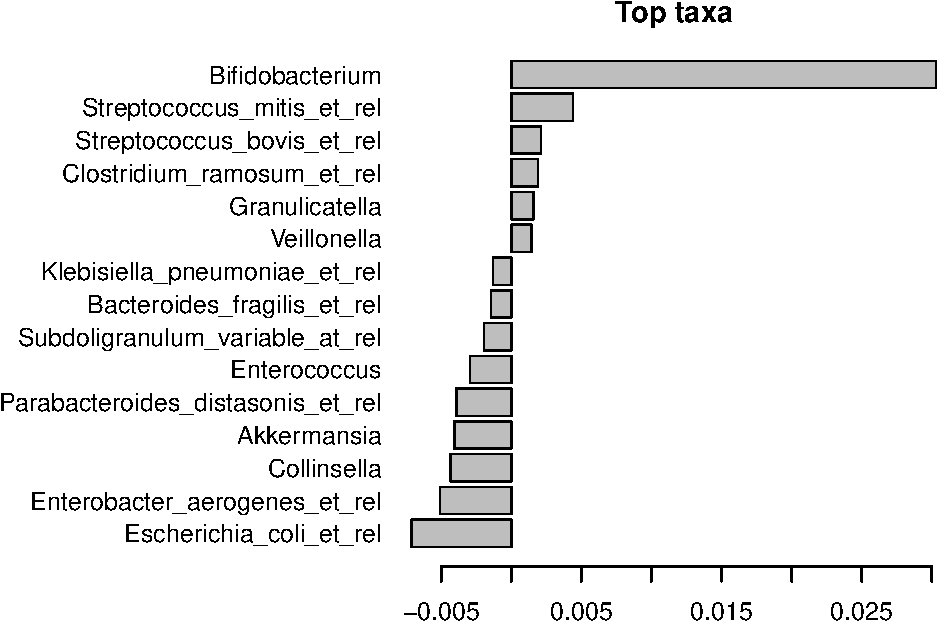
\includegraphics{results_files/figure-latex/unnamed-chunk-5-1.pdf}
\caption{Top Taxa that differ most as a function of each predictor. CC =
childcare.}
\end{figure}

\subsection{3.3 Hierarchical linear
models}\label{hierarchical-linear-models}

\subsubsection{3.3.1 Differential abundance with
LME}\label{differential-abundance-with-lme}

We evaluated the model assumptions of homogeneity of variance and
normality of residuals individually for each model by visual inspection
of residual- and quantile-quantile plots. Importantly, most of our
models showed moderate violations of the homogeneity of variance and
normality of residual assumptions. Several models violated both model
assumptions severely. In contrast, the Bayesian generalized linear
models that will be described (3.2.2) are more flexible and seem more
appropriate to model the skewed and long tailed distributions of
clr-transformed bacterial abundance.

We set contrasts in R such that the intercept reflects the CC group at
timepoint ``post'' and the coefficients of the the model (cc and time)
reflect the desired group comparisons. In the frequentist paradigm, our
hypothesis would predict that both coefficients are significantly
different from zero for more bacterial genus abundances than expected by
chance. We adjusted for multiple testing based on @benjamini1995
allowing for 20\% of false discoveries. Table x shows all coefficients
(incl. covariates) that remained significant after adjusting for
multiple testing (\(q\leq.2\)). The LMEs indicate a small signal of CC
on the abundance of some genera.

\begin{Shaded}
\begin{Highlighting}[]
\KeywordTok{library}\NormalTok{(papaja)}
\KeywordTok{library}\NormalTok{(knitr)}
\KeywordTok{library}\NormalTok{(kableExtra)}
\NormalTok{pm_table}
\end{Highlighting}
\end{Shaded}

\begin{verbatim}
##   Model Parameter Sum of Squares Mean Sum of Squares     F  Df     p
## 1            time         58.444              58.444 1.469   1  0.12
## 2              cc         52.636              52.636 1.323   1 0.181
## 3         age_d_s         79.553              79.553     2   1 0.026
## 4      bf_count_s        197.060              197.06 4.954   1 0.001
## 5         time:cc         36.229              36.229 0.911   1 0.505
## 6       Residuals       7558.549              39.782     - 190     -
## 7           Total       7982.471                   -     - 195     -
##   R Square
## 1    0.007
## 2    0.007
## 3    0.010
## 4    0.025
## 5    0.005
## 6    0.947
## 7    1.000
\end{verbatim}

\begin{Shaded}
\begin{Highlighting}[]
\KeywordTok{apa_table}\NormalTok{(pm_table)}
\end{Highlighting}
\end{Shaded}

\begin{verbatim}
## 
## 
## \begin{table}[tbp]
## \begin{center}
## \begin{threeparttable}
## \caption{\label{tab:unnamed-chunk-6}}
## \begin{tabular}{lllllll}
## \toprule
## Model Parameter & \multicolumn{1}{c}{Sum of Squares} & \multicolumn{1}{c}{Mean Sum of Squares} & \multicolumn{1}{c}{F} & \multicolumn{1}{c}{Df} & \multicolumn{1}{c}{p} & \multicolumn{1}{c}{R Square}\\
## \midrule
## time & 58.44 & 58.444 & 1.469 & 1.00 & 0.12 & 0.01\\
## cc & 52.64 & 52.636 & 1.323 & 1.00 & 0.181 & 0.01\\
## age\_d\_s & 79.55 & 79.553 & 2 & 1.00 & 0.026 & 0.01\\
## bf\_count\_s & 197.06 & 197.06 & 4.954 & 1.00 & 0.001 & 0.02\\
## time:cc & 36.23 & 36.229 & 0.911 & 1.00 & 0.505 & 0.00\\
## Residuals & 7,558.55 & 39.782 & - & 190.00 & - & 0.95\\
## Total & 7,982.47 & - & - & 195.00 & - & 1.00\\
## \bottomrule
## \end{tabular}
## \end{threeparttable}
## \end{center}
## \end{table}
\end{verbatim}

\begin{Shaded}
\begin{Highlighting}[]
\NormalTok{comp_all_df <-}\StringTok{ }\NormalTok{comp_all_df }\OperatorTok\StringTok{ }\KeywordTok{arrange}\NormalTok{(comparison)}

\KeywordTok{kable}\NormalTok{(comp_all_df, }\StringTok{"latex"}\NormalTok{, }\DataTypeTok{caption =} \StringTok{"Comparison of mu between groups"}\NormalTok{,}
  \DataTypeTok{booktabs =}\NormalTok{ T) }\OperatorTok
\StringTok{    }\KeywordTok{kable_styling}\NormalTok{() }\OperatorTok
\StringTok{    }\KeywordTok{group_rows}\NormalTok{(}\StringTok{"Age"}\NormalTok{, }\DecValTok{1}\NormalTok{, }\DecValTok{20}\NormalTok{) }\OperatorTok
\StringTok{    }\KeywordTok{group_rows}\NormalTok{(}\StringTok{"Breastfeeding"}\NormalTok{, }\DecValTok{21}\NormalTok{, }\DecValTok{25}\NormalTok{)}
\end{Highlighting}
\end{Shaded}

\begin{table}[t]

\caption{\label{tab:unnamed-chunk-6}Comparison of mu between groups}
\centering
\begin{tabular}{lrrrrl}
\toprule
comparison & mean & lower & upper & prob & genus\\
\midrule
\addlinespace[0.3em]
\multicolumn{6}{l}{\textbf{Age}}\\
\hspace{1em}age & -0.0322475 & -0.1067309 & 0.0458077 & 0.801075 & Actinomycetaceae\\
\hspace{1em}age & 0.0527438 & -0.0201235 & 0.1215064 & 0.073400 & Aerococcus\\
\hspace{1em}age & -0.0179310 & -0.0444726 & 0.0090222 & 0.906600 & Aeromonas\\
\hspace{1em}age & -0.0294980 & -0.1211939 & 0.0603634 & 0.741300 & Akkermansia\\
\hspace{1em}age & -0.0255466 & -0.0675923 & 0.0159011 & 0.887500 & Alcaligenesfaecalisetrel\\
\hspace{1em}age & -0.0521341 & -0.1093420 & 0.0061089 & 0.962200 & Allistipesetrel\\
\hspace{1em}age & -0.0283239 & -0.0596302 & 0.0030984 & 0.963025 & Anaerobiospirillum\\
\hspace{1em}age & 0.0026660 & -0.0462504 & 0.0510208 & 0.453275 & Anaerofustis\\
\hspace{1em}age & 0.0076369 & -0.0579420 & 0.0741669 & 0.409650 & Anaerostipescaccaeetrel\\
\hspace{1em}age & -0.0104363 & -0.0334147 & 0.0134173 & 0.809325 & Anaerotruncuscolihominisetrel\\
\hspace{1em}age & 0.0009257 & -0.0396629 & 0.0397777 & 0.482325 & Anaerovoraxodorimutansetrel\\
\hspace{1em}age & -0.0096374 & -0.0347590 & 0.0145815 & 0.778775 & Aneurinibacillus\\
\hspace{1em}age & -0.0569183 & -0.0966163 & -0.0159325 & 0.996850 & Aquabacterium\\
\hspace{1em}age & -0.0133486 & -0.0363521 & 0.0101089 & 0.873900 & Asteroleplasmaetrel\\
\hspace{1em}age & -0.0450606 & -0.0771109 & -0.0137424 & 0.996750 & Bacillus\\
\hspace{1em}age & -0.0166799 & -0.1149051 & 0.0878193 & 0.637250 & Bacteroidesfragilisetrel\\
\hspace{1em}age & -0.0473330 & -0.1021340 & 0.0087002 & 0.952600 & Bacteroidesintestinalisetrel\\
\hspace{1em}age & -0.0445769 & -0.1149947 & 0.0277532 & 0.888400 & Bacteroidesovatusetrel\\
\hspace{1em}age & -0.0411351 & -0.0880522 & 0.0056354 & 0.957475 & Bacteroidesplebeiusetrel\\
\hspace{1em}age & -0.0341478 & -0.0684289 & -0.0013961 & 0.977275 & Bacteroidessplachnicusetrel\\
\addlinespace[0.3em]
\multicolumn{6}{l}{\textbf{Breastfeeding}}\\
\hspace{1em}age & -0.0413594 & -0.0808608 & 0.0003953 & 0.977125 & Bacteroidesstercorisetrel\\
\hspace{1em}age & -0.0346522 & -0.1224964 & 0.0540577 & 0.785250 & Bacteroidesuniformisetrel\\
\hspace{1em}age & -0.0421769 & -0.1675406 & 0.0799988 & 0.751800 & Bacteroidesvulgatusetrel\\
\hspace{1em}age & -0.0917980 & -0.2657059 & 0.0888700 & 0.846325 & Bifidobacterium\\
\hspace{1em}age & -0.0252226 & -0.0525612 & 0.0010603 & 0.966300 & Bilophilaetrel\\
age & -0.0066925 & -0.0339682 & 0.0195620 & 0.688175 & Brachyspira\\
age & 0.0291910 & -0.0322600 & 0.0915677 & 0.175700 & Bryantellaformatexigensetrel\\
age & -0.0271341 & -0.0753811 & 0.0233852 & 0.862825 & Bulleidiamooreietrel\\
age & -0.0790701 & -0.1618650 & 0.0010880 & 0.970425 & Burkholderia\\
age & -0.0087939 & -0.0317142 & 0.0138210 & 0.780025 & Campylobacter\\
age & -0.0214210 & -0.0424097 & -0.0009025 & 0.977250 & Clostridiumcellulosietrel\\
age & -0.0122520 & -0.0350221 & 0.0096257 & 0.858850 & Clostridiumcolinumetrel\\
age & -0.0046310 & -0.0863117 & 0.0789585 & 0.541850 & Clostridiumdifficileetrel\\
age & -0.0191654 & -0.0418997 & 0.0032304 & 0.954525 & Clostridiumfelsineumetrel\\
age & -0.0073150 & -0.0494394 & 0.0354963 & 0.633125 & Clostridiumleptumetrel\\
age & -0.0035319 & -0.0595272 & 0.0520426 & 0.549900 & Clostridiumorbiscindensetrel\\
age & 0.0060026 & -0.0920970 & 0.0985439 & 0.444125 & Clostridiumramosumetrel\\
age & 0.0449726 & -0.0356547 & 0.1233454 & 0.132225 & Clostridiumsensustricto\\
age & 0.0122540 & -0.0262963 & 0.0510914 & 0.267150 & Clostridiumsphenoidesetrel\\
age & -0.0369770 & -0.0669962 & -0.0078347 & 0.993325 & Clostridiumstercorariumetrel\\
age & 0.0385096 & -0.0147057 & 0.0897579 & 0.075350 & Clostridiumsymbiosumetrel\\
age & -0.0222484 & -0.0463215 & 0.0015739 & 0.963675 & Clostridiumthermocellumetrel\\
age & -0.0803421 & -0.2326696 & 0.0704158 & 0.855975 & Collinsella\\
age & -0.0267265 & -0.0586701 & 0.0052510 & 0.949175 & Coprobacilluscatenaformisetrel\\
age & 0.0356865 & -0.0322667 & 0.1043238 & 0.151300 & Coprococcuseutactusetrel\\
age & -0.0628704 & -0.1101462 & -0.0139812 & 0.993375 & Corynebacterium\\
age & -0.0259504 & -0.0593647 & 0.0069217 & 0.937950 & Desulfovibrioetrel\\
age & -0.0101323 & -0.0335226 & 0.0120286 & 0.810225 & Dialister\\
age & 0.0258282 & -0.0410088 & 0.0949632 & 0.224875 & Doreaformicigeneransetrel\\
age & -0.0275933 & -0.1372484 & 0.0804536 & 0.691900 & Eggerthellalentaetrel\\
age & -0.0650985 & -0.1978826 & 0.0644075 & 0.838625 & Enterobacteraerogenesetrel\\
age & 0.2103005 & 0.0010579 & 0.4219027 & 0.024650 & Enterococcus\\
age & -0.0253141 & -0.1667674 & 0.1124008 & 0.642850 & Escherichiacolietrel\\
age & -0.0224829 & -0.0604072 & 0.0163216 & 0.879050 & Eubacteriumbiformeetrel\\
age & -0.0271455 & -0.0775703 & 0.0241278 & 0.854800 & Eubacteriumcylindroidesetrel\\
age & 0.0209631 & -0.0599760 & 0.1025784 & 0.302450 & Eubacteriumhalliietrel\\
age & -0.0249687 & -0.1125785 & 0.0556520 & 0.716675 & Eubacteriumlimosumetrel\\
age & 0.1132238 & 0.0066216 & 0.2214038 & 0.019300 & Eubacteriumrectaleetrel\\
age & -0.0068591 & -0.0282413 & 0.0156063 & 0.730950 & Eubacteriumsiraeumetrel\\
age & -0.0200164 & -0.0525543 & 0.0140923 & 0.883400 & Eubacteriumventriosumetrel\\
age & -0.0383667 & -0.0681528 & -0.0081708 & 0.993400 & Faecalibacteriumprausnitziietrel\\
age & -0.0091724 & -0.0335690 & 0.0150828 & 0.770175 & Fusobacteria\\
age & 0.1067825 & 0.0405352 & 0.1763443 & 0.001425 & Gemella\\
age & 0.4246822 & 0.1451230 & 0.6847421 & 0.001875 & Granulicatella\\
age & -0.0273094 & -0.0930226 & 0.0367174 & 0.796300 & Haemophilus\\
age & -0.0180381 & -0.0414719 & 0.0053187 & 0.932750 & Helicobacter\\
age & -0.0356402 & -0.1586039 & 0.0834505 & 0.715425 & Klebisiellapneumoniaeetrel\\
age & -0.0120247 & -0.0546038 & 0.0312976 & 0.712525 & Lachnobacillusbovisetrel\\
age & -0.0012059 & -0.0385595 & 0.0360372 & 0.531925 & Lachnospirapectinoschizaetrel\\
age & -0.0213857 & -0.0445313 & 0.0011411 & 0.963875 & Lactobacilluscatenaformisetrel\\
age & -0.0129269 & -0.0912476 & 0.0646138 & 0.622975 & Lactobacillusgasserietrel\\
age & -0.0392287 & -0.1761807 & 0.1087021 & 0.708150 & Lactobacillusplantarumetrel\\
age & -0.0047679 & -0.0761843 & 0.0625161 & 0.546650 & Lactobacillussalivariusetrel\\
age & -0.0223461 & -0.0750057 & 0.0310176 & 0.796325 & Lactococcus\\
age & -0.0358789 & -0.0706251 & -0.0017115 & 0.979650 & Leminorella\\
age & -0.0135652 & -0.0351573 & 0.0090174 & 0.887100 & Megamonashypermegaleetrel\\
age & -0.0215290 & -0.0539713 & 0.0096199 & 0.908425 & Megasphaeraelsdeniietrel\\
age & -0.0179559 & -0.0434247 & 0.0080430 & 0.914625 & Methylobacterium\\
age & 0.0076016 & -0.0536006 & 0.0649930 & 0.395350 & Micrococcaceae\\
age & -0.0255750 & -0.0527564 & 0.0015497 & 0.967975 & Mitsuokellamultiacidaetrel\\
age & -0.0390732 & -0.0805340 & 0.0026810 & 0.966450 & Moraxellaceae\\
age & -0.0131156 & -0.0429280 & 0.0153277 & 0.814350 & Novosphingobium\\
age & -0.0278613 & -0.0705353 & 0.0121246 & 0.909950 & Oceanospirillum\\
age & -0.0043773 & -0.0320534 & 0.0234081 & 0.620825 & Oscillospiraguillermondiietrel\\
age & -0.0504880 & -0.1052404 & 0.0037411 & 0.963875 & Oxalobacterformigenesetrel\\
age & -0.0066126 & -0.0397686 & 0.0272371 & 0.653550 & Papillibactercinnamivoransetrel\\
age & -0.0583030 & -0.1524787 & 0.0335067 & 0.892450 & Parabacteroidesdistasonisetrel\\
age & -0.0093774 & -0.0533241 & 0.0334698 & 0.666175 & Peptococcusnigeretrel\\
age & -0.0172430 & -0.0634221 & 0.0274432 & 0.772225 & Peptostreptococcusanaerobiusetrel\\
age & -0.0223036 & -0.0602890 & 0.0162404 & 0.877700 & Peptostreptococcusmicrosetrel\\
age & -0.0121066 & -0.0345856 & 0.0113448 & 0.851550 & Phascolarctobacteriumfaeciumetrel\\
age & -0.0331060 & -0.0813342 & 0.0141344 & 0.913400 & Prevotellamelaninogenicaetrel\\
age & -0.0431870 & -0.0906894 & 0.0021893 & 0.965775 & Prevotellaoralisetrel\\
age & -0.0195030 & -0.0534562 & 0.0135406 & 0.875300 & Prevotellaruminicolaetrel\\
age & -0.0503370 & -0.1102375 & 0.0112684 & 0.949050 & Prevotellatanneraeetrel\\
age & -0.0389574 & -0.1004161 & 0.0212485 & 0.896525 & Propionibacterium\\
age & -0.0421232 & -0.0978853 & 0.0133319 & 0.933725 & Proteusetrel\\
age & -0.0174237 & -0.0589727 & 0.0246632 & 0.792150 & Pseudomonas\\
age & -0.0151754 & -0.0522597 & 0.0208405 & 0.793050 & Roseburiaintestinalisetrel\\
age & -0.0321349 & -0.0670266 & 0.0037997 & 0.962950 & Ruminococcusbromiietrel\\
age & -0.0091347 & -0.0351294 & 0.0164061 & 0.761300 & Ruminococcuscallidusetrel\\
age & -0.0063009 & -0.0803697 & 0.0683158 & 0.563925 & Ruminococcusgnavusetrel\\
age & 0.0262798 & -0.0442923 & 0.0932839 & 0.222875 & Ruminococcusobeumetrel\\
age & -0.0280816 & -0.1598693 & 0.1093445 & 0.666550 & Serratia\\
age & -0.0145687 & -0.0594880 & 0.0282897 & 0.744275 & Sporobactertermitidisetrel\\
age & 0.0547383 & -0.0701229 & 0.1783251 & 0.188375 & Staphylococcus\\
age & 0.2745233 & -0.0629874 & 0.6229720 & 0.057675 & Streptococcusbovisetrel\\
age & 0.1987927 & 0.0554336 & 0.3481316 & 0.003925 & Streptococcusintermediusetrel\\
age & 0.4666311 & 0.1689220 & 0.7569542 & 0.000700 & Streptococcusmitisetrel\\
age & -0.0055580 & -0.0650090 & 0.0554671 & 0.570900 & Subdoligranulumvariableatrel\\
age & -0.0449102 & -0.0771583 & -0.0109946 & 0.995500 & Sutterellawadsworthiaetrel\\
age & -0.0599012 & -0.1190362 & 0.0001385 & 0.974525 & Tannerellaetrel\\
age & -0.0311403 & -0.0710182 & 0.0092689 & 0.937275 & UnculturedBacteroidetes\\
age & -0.0143792 & -0.0447385 & 0.0173279 & 0.819475 & UnculturedClostridialesII\\
age & -0.0135614 & -0.0349607 & 0.0076508 & 0.896400 & UnculturedMollicutes\\
age & -0.0002750 & -0.0215210 & 0.0220123 & 0.508500 & UnculturedSelenomonadaceae\\
age & 0.0674675 & -0.0354718 & 0.1703257 & 0.096575 & Veillonella\\
age & -0.0712036 & -0.1187987 & -0.0235937 & 0.998825 & Vibrio\\
age & 0.0271977 & -0.0245375 & 0.0812621 & 0.151975 & Weissellaetrel\\
age & -0.0562528 & -0.1120489 & 0.0007893 & 0.974425 & Wissellaetrel\\
age & -0.0438773 & -0.0988855 & 0.0121050 & 0.940450 & Xanthomonadaceae\\
age & -0.0610558 & -0.1405752 & 0.0200078 & 0.935650 & Yersiniaetrel\\
bf & -0.0203852 & -0.0718409 & 0.0297658 & 0.787725 & Actinomycetaceae\\
bf & -0.0682435 & -0.1117078 & -0.0227597 & 0.997800 & Aerococcus\\
bf & 0.0004459 & -0.0154459 & 0.0168790 & 0.475475 & Aeromonas\\
bf & -0.0310185 & -0.0932837 & 0.0317499 & 0.838800 & Akkermansia\\
bf & -0.0042176 & -0.0288490 & 0.0209606 & 0.630950 & Alcaligenesfaecalisetrel\\
bf & 0.0339034 & -0.0016887 & 0.0683077 & 0.027200 & Allistipesetrel\\
bf & 0.0178353 & -0.0011369 & 0.0375856 & 0.035625 & Anaerobiospirillum\\
bf & -0.0220008 & -0.0527622 & 0.0071933 & 0.924750 & Anaerofustis\\
bf & -0.0316844 & -0.0699270 & 0.0049307 & 0.951075 & Anaerostipescaccaeetrel\\
bf & -0.0052431 & -0.0192640 & 0.0097014 & 0.765175 & Anaerotruncuscolihominisetrel\\
bf & -0.0154680 & -0.0394011 & 0.0080257 & 0.898800 & Anaerovoraxodorimutansetrel\\
bf & -0.0116562 & -0.0267823 & 0.0032770 & 0.935400 & Aneurinibacillus\\
bf & -0.0067165 & -0.0321727 & 0.0182763 & 0.700100 & Aquabacterium\\
bf & 0.0021658 & -0.0127279 & 0.0170831 & 0.385550 & Asteroleplasmaetrel\\
bf & -0.0138892 & -0.0336103 & 0.0058895 & 0.916775 & Bacillus\\
bf & 0.0524269 & -0.0147732 & 0.1205980 & 0.059250 & Bacteroidesfragilisetrel\\
bf & 0.0346986 & 0.0010716 & 0.0687426 & 0.020325 & Bacteroidesintestinalisetrel\\
bf & 0.0401003 & -0.0063190 & 0.0869832 & 0.045175 & Bacteroidesovatusetrel\\
bf & 0.0292878 & 0.0000721 & 0.0580685 & 0.021375 & Bacteroidesplebeiusetrel\\
bf & 0.0193697 & -0.0013390 & 0.0397464 & 0.032325 & Bacteroidessplachnicusetrel\\
bf & 0.0258982 & 0.0011170 & 0.0511611 & 0.020050 & Bacteroidesstercorisetrel\\
bf & 0.0539003 & -0.0032907 & 0.1126092 & 0.029400 & Bacteroidesuniformisetrel\\
bf & 0.0467876 & -0.0302311 & 0.1286774 & 0.117150 & Bacteroidesvulgatusetrel\\
bf & 0.0844294 & -0.0185274 & 0.1862664 & 0.054150 & Bifidobacterium\\
bf & -0.0017534 & -0.0188501 & 0.0141000 & 0.579025 & Bilophilaetrel\\
bf & -0.0029602 & -0.0188075 & 0.0132527 & 0.646525 & Brachyspira\\
bf & 0.0036173 & -0.0378227 & 0.0443932 & 0.436225 & Bryantellaformatexigensetrel\\
bf & -0.0577602 & -0.0925012 & -0.0229302 & 0.999425 & Bulleidiamooreietrel\\
bf & 0.0163337 & -0.0272337 & 0.0599047 & 0.229200 & Burkholderia\\
bf & -0.0035987 & -0.0179638 & 0.0105807 & 0.695700 & Campylobacter\\
bf & -0.0020492 & -0.0155662 & 0.0110166 & 0.624825 & Clostridiumcellulosietrel\\
bf & -0.0058215 & -0.0199491 & 0.0085625 & 0.791575 & Clostridiumcolinumetrel\\
bf & -0.0841986 & -0.1453515 & -0.0236291 & 0.995100 & Clostridiumdifficileetrel\\
bf & -0.0032138 & -0.0173567 & 0.0113403 & 0.673300 & Clostridiumfelsineumetrel\\
bf & 0.0133744 & -0.0118667 & 0.0389263 & 0.150225 & Clostridiumleptumetrel\\
bf & -0.0188814 & -0.0555080 & 0.0172859 & 0.846675 & Clostridiumorbiscindensetrel\\
bf & -0.0007215 & -0.0636999 & 0.0634703 & 0.521175 & Clostridiumramosumetrel\\
bf & -0.0374360 & -0.0900037 & 0.0142004 & 0.919275 & Clostridiumsensustricto\\
bf & -0.0170390 & -0.0408184 & 0.0058296 & 0.924950 & Clostridiumsphenoidesetrel\\
bf & -0.0096195 & -0.0288419 & 0.0083438 & 0.845725 & Clostridiumstercorariumetrel\\
bf & -0.0269669 & -0.0608487 & 0.0068057 & 0.938150 & Clostridiumsymbiosumetrel\\
bf & -0.0060146 & -0.0201955 & 0.0090212 & 0.789850 & Clostridiumthermocellumetrel\\
bf & -0.1169607 & -0.2177691 & -0.0146341 & 0.986925 & Collinsella\\
bf & 0.0014974 & -0.0180143 & 0.0203908 & 0.437150 & Coprobacilluscatenaformisetrel\\
bf & -0.0371369 & -0.0834060 & 0.0095551 & 0.940875 & Coprococcuseutactusetrel\\
bf & -0.0063854 & -0.0343016 & 0.0201940 & 0.676600 & Corynebacterium\\
bf & 0.0051057 & -0.0144227 & 0.0254414 & 0.307325 & Desulfovibrioetrel\\
bf & -0.0050421 & -0.0191473 & 0.0097369 & 0.757150 & Dialister\\
bf & -0.0274442 & -0.0702304 & 0.0165700 & 0.890175 & Doreaformicigeneransetrel\\
bf & -0.0963302 & -0.1654071 & -0.0282099 & 0.996900 & Eggerthellalentaetrel\\
bf & 0.0446777 & -0.0479047 & 0.1339595 & 0.162675 & Enterobacteraerogenesetrel\\
bf & -0.1358867 & -0.2828903 & 0.0110059 & 0.971375 & Enterococcus\\
bf & 0.0828005 & -0.0093106 & 0.1742278 & 0.032975 & Escherichiacolietrel\\
bf & -0.0123041 & -0.0357357 & 0.0105525 & 0.852825 & Eubacteriumbiformeetrel\\
bf & -0.0054468 & -0.0363075 & 0.0264568 & 0.633425 & Eubacteriumcylindroidesetrel\\
bf & -0.0399174 & -0.0915046 & 0.0129412 & 0.929850 & Eubacteriumhalliietrel\\
bf & -0.0002311 & -0.0553942 & 0.0547507 & 0.515450 & Eubacteriumlimosumetrel\\
bf & 0.0127471 & -0.0540098 & 0.0809584 & 0.358800 & Eubacteriumrectaleetrel\\
bf & -0.0007462 & -0.0141593 & 0.0126033 & 0.544350 & Eubacteriumsiraeumetrel\\
bf & -0.0052307 & -0.0249777 & 0.0138928 & 0.702150 & Eubacteriumventriosumetrel\\
bf & -0.0072581 & -0.0254786 & 0.0102424 & 0.789425 & Faecalibacteriumprausnitziietrel\\
bf & -0.0036203 & -0.0183936 & 0.0111157 & 0.690975 & Fusobacteria\\
bf & -0.0218949 & -0.0659094 & 0.0251210 & 0.828750 & Gemella\\
bf & -0.3400283 & -0.5154008 & -0.1675786 & 0.999950 & Granulicatella\\
bf & 0.0468493 & 0.0087100 & 0.0865177 & 0.007425 & Haemophilus\\
bf & -0.0052832 & -0.0200813 & 0.0098439 & 0.754925 & Helicobacter\\
bf & 0.0508367 & -0.0242235 & 0.1315258 & 0.096675 & Klebisiellapneumoniaeetrel\\
bf & -0.0108777 & -0.0365520 & 0.0151050 & 0.797600 & Lachnobacillusbovisetrel\\
bf & -0.0238870 & -0.0550953 & 0.0085279 & 0.933800 & Lachnospirapectinoschizaetrel\\
bf & -0.0001062 & -0.0147318 & 0.0146691 & 0.511875 & Lactobacilluscatenaformisetrel\\
bf & 0.0320602 & -0.0258088 & 0.0923513 & 0.140400 & Lactobacillusgasserietrel\\
bf & 0.0353075 & -0.0672331 & 0.1425786 & 0.259950 & Lactobacillusplantarumetrel\\
bf & -0.0223519 & -0.0645207 & 0.0220551 & 0.844300 & Lactobacillussalivariusetrel\\
bf & -0.0191445 & -0.0575095 & 0.0190207 & 0.838775 & Lactococcus\\
bf & 0.0095810 & -0.0118634 & 0.0310846 & 0.190600 & Leminorella\\
bf & -0.0077706 & -0.0210919 & 0.0062221 & 0.865725 & Megamonashypermegaleetrel\\
bf & -0.0033327 & -0.0238551 & 0.0159395 & 0.629525 & Megasphaeraelsdeniietrel\\
bf & -0.0007921 & -0.0165868 & 0.0153129 & 0.540350 & Methylobacterium\\
bf & -0.0235208 & -0.0593972 & 0.0126775 & 0.901200 & Micrococcaceae\\
bf & -0.0151488 & -0.0324627 & 0.0014632 & 0.958075 & Mitsuokellamultiacidaetrel\\
bf & 0.0141010 & -0.0123959 & 0.0384493 & 0.137825 & Moraxellaceae\\
bf & 0.0033804 & -0.0146549 & 0.0215006 & 0.357100 & Novosphingobium\\
bf & 0.0044907 & -0.0180817 & 0.0271894 & 0.344950 & Oceanospirillum\\
bf & -0.0048626 & -0.0211978 & 0.0116230 & 0.720150 & Oscillospiraguillermondiietrel\\
bf & -0.0296167 & -0.0624582 & 0.0048020 & 0.959000 & Oxalobacterformigenesetrel\\
bf & 0.0002308 & -0.0193108 & 0.0201305 & 0.489300 & Papillibactercinnamivoransetrel\\
bf & 0.0326778 & -0.0235664 & 0.0900521 & 0.126400 & Parabacteroidesdistasonisetrel\\
bf & -0.0154853 & -0.0493666 & 0.0173130 & 0.819225 & Peptococcusnigeretrel\\
bf & -0.0061614 & -0.0341419 & 0.0219756 & 0.668200 & Peptostreptococcusanaerobiusetrel\\
bf & -0.0000450 & -0.0217395 & 0.0221903 & 0.500350 & Peptostreptococcusmicrosetrel\\
bf & -0.0066451 & -0.0206857 & 0.0075290 & 0.824950 & Phascolarctobacteriumfaeciumetrel\\
bf & -0.0040288 & -0.0340054 & 0.0270796 & 0.602900 & Prevotellamelaninogenicaetrel\\
bf & 0.0208420 & -0.0095918 & 0.0499973 & 0.082525 & Prevotellaoralisetrel\\
bf & 0.0198902 & -0.0001007 & 0.0400267 & 0.027350 & Prevotellaruminicolaetrel\\
bf & 0.0308709 & -0.0076642 & 0.0705463 & 0.056525 & Prevotellatanneraeetrel\\
bf & 0.0149530 & -0.0252332 & 0.0540087 & 0.226325 & Propionibacterium\\
bf & 0.0317798 & -0.0021892 & 0.0659916 & 0.030750 & Proteusetrel\\
bf & 0.0030549 & -0.0239183 & 0.0285829 & 0.409150 & Pseudomonas\\
bf & -0.0133958 & -0.0350106 & 0.0078109 & 0.890300 & Roseburiaintestinalisetrel\\
bf & -0.0018653 & -0.0221275 & 0.0189081 & 0.568750 & Ruminococcusbromiietrel\\
bf & -0.0054153 & -0.0207344 & 0.0098746 & 0.758225 & Ruminococcuscallidusetrel\\
bf & -0.0274475 & -0.0739072 & 0.0216312 & 0.869450 & Ruminococcusgnavusetrel\\
bf & -0.0536224 & -0.0992725 & -0.0064896 & 0.985700 & Ruminococcusobeumetrel\\
bf & 0.0505287 & -0.0281280 & 0.1290755 & 0.096675 & Serratia\\
bf & -0.0067315 & -0.0331640 & 0.0194743 & 0.697100 & Sporobactertermitidisetrel\\
bf & 0.1136289 & 0.0338857 & 0.1949566 & 0.001550 & Staphylococcus\\
bf & 0.0742704 & -0.1527833 & 0.2914643 & 0.254425 & Streptococcusbovisetrel\\
bf & 0.0226228 & -0.0727660 & 0.1208399 & 0.323475 & Streptococcusintermediusetrel\\
bf & 0.2401225 & 0.0567160 & 0.4240907 & 0.005350 & Streptococcusmitisetrel\\
bf & -0.0204345 & -0.0604360 & 0.0175738 & 0.849075 & Subdoligranulumvariableatrel\\
bf & 0.0028590 & -0.0166725 & 0.0224108 & 0.388225 & Sutterellawadsworthiaetrel\\
bf & 0.0359606 & -0.0005474 & 0.0714070 & 0.022800 & Tannerellaetrel\\
bf & 0.0134038 & -0.0112033 & 0.0376266 & 0.138175 & UnculturedBacteroidetes\\
bf & -0.0067220 & -0.0253742 & 0.0122365 & 0.760650 & UnculturedClostridialesII\\
bf & -0.0044269 & -0.0180628 & 0.0097873 & 0.737875 & UnculturedMollicutes\\
bf & -0.0078383 & -0.0205113 & 0.0048282 & 0.890475 & UnculturedSelenomonadaceae\\
bf & 0.0666947 & 0.0105123 & 0.1244842 & 0.009025 & Veillonella\\
bf & -0.0350946 & -0.0689416 & -0.0029351 & 0.982850 & Vibrio\\
bf & 0.0038726 & -0.0255977 & 0.0346582 & 0.400550 & Weissellaetrel\\
bf & -0.0666147 & -0.1162935 & -0.0169708 & 0.995750 & Wissellaetrel\\
bf & 0.0197935 & -0.0146725 & 0.0544985 & 0.129350 & Xanthomonadaceae\\
bf & 0.0177488 & -0.0280765 & 0.0687619 & 0.235375 & Yersiniaetrel\\
ccpost\_ccpre & 0.0714808 & -0.0631054 & 0.2068813 & 0.147500 & Actinomycetaceae\\
ccpost\_ccpre & -0.0801387 & -0.2160749 & 0.0498022 & 0.882275 & Aerococcus\\
ccpost\_ccpre & 0.0676358 & 0.0208152 & 0.1158860 & 0.002850 & Aeromonas\\
ccpost\_ccpre & 0.1606566 & -0.0664404 & 0.3874318 & 0.080025 & Akkermansia\\
ccpost\_ccpre & 0.1009352 & 0.0134367 & 0.1823901 & 0.009400 & Alcaligenesfaecalisetrel\\
ccpost\_ccpre & 0.1262234 & -0.0054688 & 0.2583734 & 0.033425 & Allistipesetrel\\
ccpost\_ccpre & 0.0843550 & 0.0208711 & 0.1454646 & 0.004400 & Anaerobiospirillum\\
ccpost\_ccpre & -0.0094364 & -0.1073966 & 0.0834723 & 0.577450 & Anaerofustis\\
ccpost\_ccpre & 0.0061333 & -0.1178440 & 0.1298123 & 0.459825 & Anaerostipescaccaeetrel\\
ccpost\_ccpre & 0.0478654 & 0.0026488 & 0.0923230 & 0.018375 & Anaerotruncuscolihominisetrel\\
ccpost\_ccpre & 0.0199815 & -0.0552428 & 0.0922314 & 0.296275 & Anaerovoraxodorimutansetrel\\
ccpost\_ccpre & 0.0358804 & -0.0098497 & 0.0811284 & 0.058275 & Aneurinibacillus\\
ccpost\_ccpre & 0.1207901 & 0.0379847 & 0.2024748 & 0.002200 & Aquabacterium\\
ccpost\_ccpre & 0.0542088 & 0.0099914 & 0.0995155 & 0.008225 & Asteroleplasmaetrel\\
ccpost\_ccpre & 0.0594759 & -0.0000919 & 0.1196866 & 0.025725 & Bacillus\\
ccpost\_ccpre & 0.0901584 & -0.1569733 & 0.3362849 & 0.234350 & Bacteroidesfragilisetrel\\
ccpost\_ccpre & 0.1177834 & -0.0110737 & 0.2485991 & 0.038925 & Bacteroidesintestinalisetrel\\
ccpost\_ccpre & 0.1401911 & -0.0283054 & 0.3104586 & 0.054925 & Bacteroidesovatusetrel\\
ccpost\_ccpre & 0.1066938 & -0.0003433 & 0.2146935 & 0.027575 & Bacteroidesplebeiusetrel\\
ccpost\_ccpre & 0.0870416 & 0.0183545 & 0.1550311 & 0.006225 & Bacteroidessplachnicusetrel\\
ccpost\_ccpre & 0.1112112 & 0.0211784 & 0.2040022 & 0.008750 & Bacteroidesstercorisetrel\\
ccpost\_ccpre & 0.0929546 & -0.1261740 & 0.3085202 & 0.195475 & Bacteroidesuniformisetrel\\
ccpost\_ccpre & 0.0583966 & -0.2601799 & 0.3800344 & 0.355350 & Bacteroidesvulgatusetrel\\
ccpost\_ccpre & 0.1999627 & -0.1668816 & 0.5810293 & 0.142000 & Bifidobacterium\\
ccpost\_ccpre & 0.0539312 & 0.0044614 & 0.1044438 & 0.017875 & Bilophilaetrel\\
ccpost\_ccpre & 0.0442647 & -0.0077012 & 0.0944129 & 0.042000 & Brachyspira\\
ccpost\_ccpre & -0.0446305 & -0.1714153 & 0.0814171 & 0.756200 & Bryantellaformatexigensetrel\\
ccpost\_ccpre & 0.0675108 & -0.0252583 & 0.1621927 & 0.076750 & Bulleidiamooreietrel\\
ccpost\_ccpre & 0.1475540 & 0.0024254 & 0.2832208 & 0.019875 & Burkholderia\\
ccpost\_ccpre & 0.0594561 & 0.0160049 & 0.1023700 & 0.003725 & Campylobacter\\
ccpost\_ccpre & 0.0559934 & 0.0153437 & 0.0963949 & 0.003350 & Clostridiumcellulosietrel\\
ccpost\_ccpre & 0.0547155 & 0.0111401 & 0.0983503 & 0.006425 & Clostridiumcolinumetrel\\
ccpost\_ccpre & 0.0020036 & -0.2099035 & 0.2072416 & 0.492575 & Clostridiumdifficileetrel\\
ccpost\_ccpre & 0.0656078 & 0.0228552 & 0.1110765 & 0.001700 & Clostridiumfelsineumetrel\\
ccpost\_ccpre & 0.0254429 & -0.0508430 & 0.1036964 & 0.259700 & Clostridiumleptumetrel\\
ccpost\_ccpre & 0.0482368 & -0.0759243 & 0.1696519 & 0.219300 & Clostridiumorbiscindensetrel\\
ccpost\_ccpre & 0.1097282 & -0.1177290 & 0.3469967 & 0.175300 & Clostridiumramosumetrel\\
ccpost\_ccpre & -0.0412507 & -0.2311893 & 0.1405503 & 0.668200 & Clostridiumsensustricto\\
ccpost\_ccpre & 0.0190983 & -0.0588569 & 0.0961676 & 0.313700 & Clostridiumsphenoidesetrel\\
ccpost\_ccpre & 0.0577960 & 0.0057885 & 0.1098734 & 0.014375 & Clostridiumstercorariumetrel\\
ccpost\_ccpre & -0.0128544 & -0.1216518 & 0.0988798 & 0.591900 & Clostridiumsymbiosumetrel\\
ccpost\_ccpre & 0.0485334 & 0.0056266 & 0.0940513 & 0.015275 & Clostridiumthermocellumetrel\\
ccpost\_ccpre & 0.0917936 & -0.2808400 & 0.4876710 & 0.314000 & Collinsella\\
ccpost\_ccpre & 0.0784669 & 0.0194983 & 0.1390347 & 0.005125 & Coprobacilluscatenaformisetrel\\
ccpost\_ccpre & 0.0220413 & -0.1181480 & 0.1722576 & 0.384200 & Coprococcuseutactusetrel\\
ccpost\_ccpre & 0.0778919 & -0.0048803 & 0.1579341 & 0.031400 & Corynebacterium\\
ccpost\_ccpre & 0.0749031 & 0.0110047 & 0.1389476 & 0.010450 & Desulfovibrioetrel\\
ccpost\_ccpre & 0.0524053 & 0.0078753 & 0.0960775 & 0.009325 & Dialister\\
ccpost\_ccpre & 0.0145512 & -0.1274918 & 0.1637568 & 0.424750 & Doreaformicigeneransetrel\\
ccpost\_ccpre & 0.0052034 & -0.1876119 & 0.1891583 & 0.475700 & Eggerthellalentaetrel\\
ccpost\_ccpre & 0.0817871 & -0.2799567 & 0.4479523 & 0.330800 & Enterobacteraerogenesetrel\\
ccpost\_ccpre & -0.4068938 & -0.9283916 & 0.0997637 & 0.945850 & Enterococcus\\
ccpost\_ccpre & 0.0645238 & -0.2606253 & 0.3862536 & 0.347700 & Escherichiacolietrel\\
ccpost\_ccpre & 0.0576674 & -0.0144851 & 0.1328907 & 0.060925 & Eubacteriumbiformeetrel\\
ccpost\_ccpre & 0.0518622 & -0.0567512 & 0.1578305 & 0.172400 & Eubacteriumcylindroidesetrel\\
ccpost\_ccpre & 0.0256582 & -0.1639141 & 0.2217767 & 0.400725 & Eubacteriumhalliietrel\\
ccpost\_ccpre & 0.1245813 & -0.0731419 & 0.3163180 & 0.104900 & Eubacteriumlimosumetrel\\
ccpost\_ccpre & -0.1114760 & -0.3346174 & 0.1178339 & 0.840600 & Eubacteriumrectaleetrel\\
ccpost\_ccpre & 0.0281503 & -0.0128652 & 0.0716455 & 0.092875 & Eubacteriumsiraeumetrel\\
ccpost\_ccpre & 0.0442474 & -0.0142374 & 0.1041693 & 0.069950 & Eubacteriumventriosumetrel\\
ccpost\_ccpre & 0.0322825 & -0.0268478 & 0.0907553 & 0.138975 & Faecalibacteriumprausnitziietrel\\
ccpost\_ccpre & 0.0349176 & -0.0093832 & 0.0806214 & 0.061725 & Fusobacteria\\
ccpost\_ccpre & -0.0389345 & -0.1804335 & 0.0970836 & 0.711100 & Gemella\\
ccpost\_ccpre & -0.7479270 & -1.3746785 & -0.1215390 & 0.989925 & Granulicatella\\
ccpost\_ccpre & 0.0357982 & -0.1176098 & 0.1894532 & 0.318325 & Haemophilus\\
ccpost\_ccpre & 0.0686879 & 0.0246026 & 0.1135953 & 0.001675 & Helicobacter\\
ccpost\_ccpre & 0.0717130 & -0.2496744 & 0.4036311 & 0.336475 & Klebisiellapneumoniaeetrel\\
ccpost\_ccpre & 0.0153718 & -0.0647399 & 0.0942158 & 0.349925 & Lachnobacillusbovisetrel\\
ccpost\_ccpre & 0.0340041 & -0.0305661 & 0.0961790 & 0.142525 & Lachnospirapectinoschizaetrel\\
ccpost\_ccpre & 0.0783473 & 0.0329770 & 0.1222359 & 0.000475 & Lactobacilluscatenaformisetrel\\
ccpost\_ccpre & 0.0726127 & -0.1130327 & 0.2602281 & 0.224300 & Lactobacillusgasserietrel\\
ccpost\_ccpre & 0.1591386 & -0.1797515 & 0.5040804 & 0.175825 & Lactobacillusplantarumetrel\\
ccpost\_ccpre & 0.0408656 & -0.1230135 & 0.2130383 & 0.320025 & Lactobacillussalivariusetrel\\
ccpost\_ccpre & 0.1024126 & 0.0040334 & 0.2036271 & 0.021850 & Lactococcus\\
ccpost\_ccpre & 0.0852075 & 0.0094441 & 0.1615542 & 0.014300 & Leminorella\\
ccpost\_ccpre & 0.0594535 & 0.0165597 & 0.1009878 & 0.002650 & Megamonashypermegaleetrel\\
ccpost\_ccpre & 0.0754205 & 0.0063127 & 0.1417160 & 0.014575 & Megasphaeraelsdeniietrel\\
ccpost\_ccpre & 0.0571828 & 0.0092593 & 0.1075583 & 0.010450 & Methylobacterium\\
ccpost\_ccpre & -0.0039749 & -0.1135023 & 0.0991350 & 0.531475 & Micrococcaceae\\
ccpost\_ccpre & 0.0584945 & 0.0069076 & 0.1109923 & 0.012525 & Mitsuokellamultiacidaetrel\\
ccpost\_ccpre & 0.0630783 & -0.0259725 & 0.1551263 & 0.083725 & Moraxellaceae\\
ccpost\_ccpre & 0.0313913 & -0.0307566 & 0.0933976 & 0.158400 & Novosphingobium\\
ccpost\_ccpre & 0.0916672 & 0.0189669 & 0.1668519 & 0.006700 & Oceanospirillum\\
ccpost\_ccpre & 0.0257998 & -0.0240211 & 0.0771031 & 0.158100 & Oscillospiraguillermondiietrel\\
ccpost\_ccpre & -0.0076832 & -0.1108270 & 0.0945791 & 0.552700 & Oxalobacterformigenesetrel\\
ccpost\_ccpre & 0.0281094 & -0.0333681 & 0.0908125 & 0.184625 & Papillibactercinnamivoransetrel\\
ccpost\_ccpre & 0.1333020 & -0.1011676 & 0.3618622 & 0.127275 & Parabacteroidesdistasonisetrel\\
ccpost\_ccpre & 0.0226588 & -0.0488780 & 0.0888971 & 0.254125 & Peptococcusnigeretrel\\
ccpost\_ccpre & 0.0870626 & -0.0079699 & 0.1813098 & 0.034425 & Peptostreptococcusanaerobiusetrel\\
ccpost\_ccpre & 0.0752944 & 0.0033492 & 0.1472719 & 0.020700 & Peptostreptococcusmicrosetrel\\
ccpost\_ccpre & 0.0531838 & 0.0091187 & 0.0953973 & 0.006500 & Phascolarctobacteriumfaeciumetrel\\
ccpost\_ccpre & 0.0495202 & -0.0625353 & 0.1572032 & 0.187550 & Prevotellamelaninogenicaetrel\\
ccpost\_ccpre & 0.0984074 & -0.0089990 & 0.2095339 & 0.040625 & Prevotellaoralisetrel\\
ccpost\_ccpre & 0.0525344 & -0.0125472 & 0.1205968 & 0.060600 & Prevotellaruminicolaetrel\\
ccpost\_ccpre & 0.1221535 & -0.0269516 & 0.2672303 & 0.055150 & Prevotellatanneraeetrel\\
ccpost\_ccpre & 0.0991198 & -0.0550108 & 0.2487824 & 0.098600 & Propionibacterium\\
ccpost\_ccpre & 0.0689298 & -0.0620275 & 0.1952277 & 0.146725 & Proteusetrel\\
ccpost\_ccpre & 0.0571436 & -0.0324563 & 0.1578189 & 0.116625 & Pseudomonas\\
ccpost\_ccpre & 0.0224613 & -0.0401437 & 0.0843668 & 0.238675 & Roseburiaintestinalisetrel\\
ccpost\_ccpre & 0.0345471 & -0.0291732 & 0.0960084 & 0.136650 & Ruminococcusbromiietrel\\
ccpost\_ccpre & 0.0411107 & -0.0065300 & 0.0887901 & 0.044075 & Ruminococcuscallidusetrel\\
ccpost\_ccpre & 0.0573634 & -0.1138672 & 0.2334883 & 0.259175 & Ruminococcusgnavusetrel\\
ccpost\_ccpre & 0.0102241 & -0.1430270 & 0.1591482 & 0.447475 & Ruminococcusobeumetrel\\
ccpost\_ccpre & 0.0798164 & -0.2377062 & 0.3883290 & 0.301275 & Serratia\\
ccpost\_ccpre & 0.0476262 & -0.0346059 & 0.1316717 & 0.129275 & Sporobactertermitidisetrel\\
ccpost\_ccpre & -0.1657218 & -0.4627001 & 0.1211997 & 0.868675 & Staphylococcus\\
ccpost\_ccpre & -0.8918626 & -1.6480581 & -0.1149039 & 0.989200 & Streptococcusbovisetrel\\
ccpost\_ccpre & -0.3281082 & -0.6338225 & -0.0050605 & 0.979225 & Streptococcusintermediusetrel\\
ccpost\_ccpre & -0.6614228 & -1.3768538 & 0.0459848 & 0.966450 & Streptococcusmitisetrel\\
ccpost\_ccpre & 0.0052418 & -0.1282212 & 0.1338490 & 0.467400 & Subdoligranulumvariableatrel\\
ccpost\_ccpre & 0.0658101 & 0.0054016 & 0.1236245 & 0.014700 & Sutterellawadsworthiaetrel\\
ccpost\_ccpre & 0.1441700 & -0.0000441 & 0.2820914 & 0.025275 & Tannerellaetrel\\
ccpost\_ccpre & 0.0826191 & -0.0051041 & 0.1743551 & 0.036400 & UnculturedBacteroidetes\\
ccpost\_ccpre & 0.0106001 & -0.0463051 & 0.0673030 & 0.356650 & UnculturedClostridialesII\\
ccpost\_ccpre & 0.0575455 & 0.0166846 & 0.0978018 & 0.003175 & UnculturedMollicutes\\
ccpost\_ccpre & 0.0408953 & -0.0002178 & 0.0808911 & 0.023275 & UnculturedSelenomonadaceae\\
ccpost\_ccpre & -0.0576760 & -0.2549867 & 0.1329568 & 0.721625 & Veillonella\\
ccpost\_ccpre & 0.0497697 & -0.0372907 & 0.1332843 & 0.126150 & Vibrio\\
ccpost\_ccpre & -0.0267411 & -0.1197371 & 0.0650920 & 0.715725 & Weissellaetrel\\
ccpost\_ccpre & 0.1019583 & 0.0152321 & 0.1878860 & 0.012175 & Wissellaetrel\\
ccpost\_ccpre & 0.1254913 & 0.0131599 & 0.2338538 & 0.013175 & Xanthomonadaceae\\
ccpost\_ccpre & 0.0883462 & -0.1102060 & 0.2852167 & 0.187575 & Yersiniaetrel\\
ccpost\_noccpost & 0.1010320 & -0.0099225 & 0.2089173 & 0.035825 & Actinomycetaceae\\
ccpost\_noccpost & -0.0301070 & -0.1378624 & 0.0752272 & 0.707850 & Aerococcus\\
ccpost\_noccpost & 0.0587984 & 0.0178811 & 0.1002335 & 0.003025 & Aeromonas\\
ccpost\_noccpost & 0.1060052 & -0.0546838 & 0.2714458 & 0.098950 & Akkermansia\\
ccpost\_noccpost & 0.0860542 & 0.0173524 & 0.1521327 & 0.007000 & Alcaligenesfaecalisetrel\\
ccpost\_noccpost & 0.0261468 & -0.0688189 & 0.1211528 & 0.288775 & Allistipesetrel\\
ccpost\_noccpost & 0.0389819 & -0.0111090 & 0.0895958 & 0.063100 & Anaerobiospirillum\\
ccpost\_noccpost & 0.0072218 & -0.0711656 & 0.0832719 & 0.426825 & Anaerofustis\\
ccpost\_noccpost & -0.0234731 & -0.1295537 & 0.0765524 & 0.668600 & Anaerostipescaccaeetrel\\
ccpost\_noccpost & 0.0442848 & 0.0082638 & 0.0824382 & 0.008975 & Anaerotruncuscolihominisetrel\\
ccpost\_noccpost & 0.0173138 & -0.0434521 & 0.0779461 & 0.284200 & Anaerovoraxodorimutansetrel\\
ccpost\_noccpost & 0.0599054 & 0.0224251 & 0.0970679 & 0.000900 & Aneurinibacillus\\
ccpost\_noccpost & 0.1105619 & 0.0441310 & 0.1758924 & 0.000350 & Aquabacterium\\
ccpost\_noccpost & 0.0508013 & 0.0117614 & 0.0888599 & 0.004800 & Asteroleplasmaetrel\\
ccpost\_noccpost & 0.0624478 & 0.0130933 & 0.1127802 & 0.007000 & Bacillus\\
ccpost\_noccpost & 0.0031272 & -0.1896054 & 0.1821920 & 0.477075 & Bacteroidesfragilisetrel\\
ccpost\_noccpost & 0.0411070 & -0.0522243 & 0.1338278 & 0.187775 & Bacteroidesintestinalisetrel\\
ccpost\_noccpost & 0.0124260 & -0.1128111 & 0.1359080 & 0.418050 & Bacteroidesovatusetrel\\
ccpost\_noccpost & 0.0503343 & -0.0307270 & 0.1309331 & 0.108425 & Bacteroidesplebeiusetrel\\
ccpost\_noccpost & 0.0318613 & -0.0221525 & 0.0876997 & 0.128125 & Bacteroidessplachnicusetrel\\
ccpost\_noccpost & 0.0513054 & -0.0150788 & 0.1199540 & 0.067425 & Bacteroidesstercorisetrel\\
ccpost\_noccpost & 0.0366599 & -0.1331977 & 0.2039495 & 0.326075 & Bacteroidesuniformisetrel\\
ccpost\_noccpost & 0.0078168 & -0.2350758 & 0.2366283 & 0.466550 & Bacteroidesvulgatusetrel\\
ccpost\_noccpost & 0.2503841 & -0.0583324 & 0.5615534 & 0.053925 & Bifidobacterium\\
ccpost\_noccpost & 0.0694672 & 0.0274252 & 0.1119554 & 0.000825 & Bilophilaetrel\\
ccpost\_noccpost & 0.0406995 & -0.0017076 & 0.0815727 & 0.025375 & Brachyspira\\
ccpost\_noccpost & 0.0469946 & -0.0623805 & 0.1547419 & 0.191875 & Bryantellaformatexigensetrel\\
ccpost\_noccpost & 0.0800804 & 0.0041724 & 0.1558702 & 0.020825 & Bulleidiamooreietrel\\
ccpost\_noccpost & 0.0558239 & -0.0605921 & 0.1709264 & 0.168075 & Burkholderia\\
ccpost\_noccpost & 0.0431435 & 0.0083685 & 0.0812732 & 0.009625 & Campylobacter\\
ccpost\_noccpost & 0.0592122 & 0.0269643 & 0.0922779 & 0.000325 & Clostridiumcellulosietrel\\
ccpost\_noccpost & 0.0447553 & 0.0104741 & 0.0813295 & 0.006975 & Clostridiumcolinumetrel\\
ccpost\_noccpost & 0.0273555 & -0.1315731 & 0.1894201 & 0.366700 & Clostridiumdifficileetrel\\
ccpost\_noccpost & 0.0551391 & 0.0173140 & 0.0935809 & 0.002400 & Clostridiumfelsineumetrel\\
ccpost\_noccpost & 0.0434663 & -0.0205853 & 0.1085439 & 0.096025 & Clostridiumleptumetrel\\
ccpost\_noccpost & 0.0585809 & -0.0393830 & 0.1577510 & 0.122525 & Clostridiumorbiscindensetrel\\
ccpost\_noccpost & 0.0570657 & -0.1118347 & 0.2228848 & 0.245250 & Clostridiumramosumetrel\\
ccpost\_noccpost & 0.0427728 & -0.1141141 & 0.1975784 & 0.289275 & Clostridiumsensustricto\\
ccpost\_noccpost & 0.0032165 & -0.0597378 & 0.0660735 & 0.458575 & Clostridiumsphenoidesetrel\\
ccpost\_noccpost & 0.0686714 & 0.0264718 & 0.1112198 & 0.000825 & Clostridiumstercorariumetrel\\
ccpost\_noccpost & -0.0190294 & -0.1069973 & 0.0694682 & 0.662875 & Clostridiumsymbiosumetrel\\
ccpost\_noccpost & 0.0569610 & 0.0188848 & 0.0946568 & 0.001825 & Clostridiumthermocellumetrel\\
ccpost\_noccpost & -0.0421413 & -0.3345171 & 0.2374151 & 0.606175 & Collinsella\\
ccpost\_noccpost & 0.0707372 & 0.0210234 & 0.1192607 & 0.002925 & Coprobacilluscatenaformisetrel\\
ccpost\_noccpost & 0.0170888 & -0.1036799 & 0.1371792 & 0.388550 & Coprococcuseutactusetrel\\
ccpost\_noccpost & 0.0661972 & -0.0030223 & 0.1322964 & 0.028575 & Corynebacterium\\
ccpost\_noccpost & 0.0466835 & -0.0052521 & 0.0993297 & 0.041325 & Desulfovibrioetrel\\
ccpost\_noccpost & 0.0446504 & 0.0075685 & 0.0813154 & 0.007825 & Dialister\\
ccpost\_noccpost & -0.0067972 & -0.1246627 & 0.1081854 & 0.543200 & Doreaformicigeneransetrel\\
ccpost\_noccpost & 0.0688092 & -0.0868637 & 0.2203462 & 0.187100 & Eggerthellalentaetrel\\
ccpost\_noccpost & 0.0413057 & -0.2411779 & 0.3105011 & 0.377450 & Enterobacteraerogenesetrel\\
ccpost\_noccpost & -0.0726777 & -0.4731339 & 0.3149178 & 0.640325 & Enterococcus\\
ccpost\_noccpost & -0.0036744 & -0.2465897 & 0.2376812 & 0.502500 & Escherichiacolietrel\\
ccpost\_noccpost & 0.0683728 & 0.0107285 & 0.1268947 & 0.010600 & Eubacteriumbiformeetrel\\
ccpost\_noccpost & 0.0882326 & 0.0039166 & 0.1737892 & 0.021500 & Eubacteriumcylindroidesetrel\\
ccpost\_noccpost & -0.0110965 & -0.1520177 & 0.1311736 & 0.555500 & Eubacteriumhalliietrel\\
ccpost\_noccpost & 0.0880077 & -0.0492708 & 0.2295639 & 0.103775 & Eubacteriumlimosumetrel\\
ccpost\_noccpost & 0.0105315 & -0.1750815 & 0.2011070 & 0.446025 & Eubacteriumrectaleetrel\\
ccpost\_noccpost & 0.0413085 & 0.0052100 & 0.0755385 & 0.010800 & Eubacteriumsiraeumetrel\\
ccpost\_noccpost & 0.0382385 & -0.0095787 & 0.0891776 & 0.064775 & Eubacteriumventriosumetrel\\
ccpost\_noccpost & 0.0734749 & 0.0310113 & 0.1175227 & 0.000425 & Faecalibacteriumprausnitziietrel\\
ccpost\_noccpost & 0.0390064 & 0.0016773 & 0.0766156 & 0.018650 & Fusobacteria\\
ccpost\_noccpost & -0.0351060 & -0.1501174 & 0.0829313 & 0.723125 & Gemella\\
ccpost\_noccpost & -0.2365313 & -0.7340680 & 0.2456657 & 0.829875 & Granulicatella\\
ccpost\_noccpost & -0.0123826 & -0.1249291 & 0.1043853 & 0.582500 & Haemophilus\\
ccpost\_noccpost & 0.0498511 & 0.0116151 & 0.0884329 & 0.005775 & Helicobacter\\
ccpost\_noccpost & 0.0511469 & -0.1807344 & 0.2800266 & 0.319675 & Klebisiellapneumoniaeetrel\\
ccpost\_noccpost & 0.0395613 & -0.0236227 & 0.1046652 & 0.113225 & Lachnobacillusbovisetrel\\
ccpost\_noccpost & 0.0318048 & -0.0234417 & 0.0839101 & 0.120000 & Lachnospirapectinoschizaetrel\\
ccpost\_noccpost & 0.0514418 & 0.0135911 & 0.0899139 & 0.004475 & Lactobacilluscatenaformisetrel\\
ccpost\_noccpost & 0.0785116 & -0.0709516 & 0.2211023 & 0.144050 & Lactobacillusgasserietrel\\
ccpost\_noccpost & 0.0632637 & -0.2089720 & 0.3259362 & 0.311750 & Lactobacillusplantarumetrel\\
ccpost\_noccpost & 0.0212578 & -0.0924887 & 0.1403614 & 0.358100 & Lactobacillussalivariusetrel\\
ccpost\_noccpost & 0.0904651 & 0.0073424 & 0.1722858 & 0.015175 & Lactococcus\\
ccpost\_noccpost & 0.0672571 & 0.0072951 & 0.1255855 & 0.013450 & Leminorella\\
ccpost\_noccpost & 0.0455745 & 0.0109546 & 0.0813560 & 0.005175 & Megamonashypermegaleetrel\\
ccpost\_noccpost & 0.0499610 & -0.0044384 & 0.1050033 & 0.036350 & Megasphaeraelsdeniietrel\\
ccpost\_noccpost & 0.0469085 & 0.0053869 & 0.0878488 & 0.011800 & Methylobacterium\\
ccpost\_noccpost & 0.0173605 & -0.0757963 & 0.1017377 & 0.348350 & Micrococcaceae\\
ccpost\_noccpost & 0.0561354 & 0.0142429 & 0.0970108 & 0.004075 & Mitsuokellamultiacidaetrel\\
ccpost\_noccpost & 0.0449236 & -0.0258135 & 0.1138438 & 0.105050 & Moraxellaceae\\
ccpost\_noccpost & 0.0433950 & -0.0063538 & 0.0926958 & 0.043200 & Novosphingobium\\
ccpost\_noccpost & 0.0434261 & -0.0228291 & 0.1135274 & 0.104850 & Oceanospirillum\\
ccpost\_noccpost & 0.0507407 & 0.0085482 & 0.0916857 & 0.008550 & Oscillospiraguillermondiietrel\\
ccpost\_noccpost & 0.0316642 & -0.0517749 & 0.1184775 & 0.234800 & Oxalobacterformigenesetrel\\
ccpost\_noccpost & 0.0327651 & -0.0168284 & 0.0860101 & 0.104900 & Papillibactercinnamivoransetrel\\
ccpost\_noccpost & 0.0468857 & -0.1245088 & 0.2091988 & 0.276700 & Parabacteroidesdistasonisetrel\\
ccpost\_noccpost & 0.0740058 & 0.0224535 & 0.1220804 & 0.001775 & Peptococcusnigeretrel\\
ccpost\_noccpost & 0.0476446 & -0.0280213 & 0.1263743 & 0.111625 & Peptostreptococcusanaerobiusetrel\\
ccpost\_noccpost & 0.0198824 & -0.0377465 & 0.0779068 & 0.248350 & Peptostreptococcusmicrosetrel\\
ccpost\_noccpost & 0.0453513 & 0.0093442 & 0.0826889 & 0.006775 & Phascolarctobacteriumfaeciumetrel\\
ccpost\_noccpost & 0.0830781 & 0.0016224 & 0.1686069 & 0.026100 & Prevotellamelaninogenicaetrel\\
ccpost\_noccpost & 0.0643010 & -0.0163434 & 0.1432596 & 0.057675 & Prevotellaoralisetrel\\
ccpost\_noccpost & 0.0430853 & -0.0103573 & 0.0951793 & 0.054250 & Prevotellaruminicolaetrel\\
ccpost\_noccpost & 0.0373514 & -0.0705737 & 0.1421272 & 0.240825 & Prevotellatanneraeetrel\\
ccpost\_noccpost & 0.0558479 & -0.0528642 & 0.1607921 & 0.147200 & Propionibacterium\\
ccpost\_noccpost & 0.0154016 & -0.0779189 & 0.1100913 & 0.371125 & Proteusetrel\\
ccpost\_noccpost & 0.0669090 & -0.0045262 & 0.1403643 & 0.035925 & Pseudomonas\\
ccpost\_noccpost & 0.0285206 & -0.0237470 & 0.0806358 & 0.138625 & Roseburiaintestinalisetrel\\
ccpost\_noccpost & 0.0636613 & 0.0141158 & 0.1127801 & 0.005950 & Ruminococcusbromiietrel\\
ccpost\_noccpost & 0.0457293 & 0.0053221 & 0.0855796 & 0.012800 & Ruminococcuscallidusetrel\\
ccpost\_noccpost & 0.0482729 & -0.0910284 & 0.1855682 & 0.243075 & Ruminococcusgnavusetrel\\
ccpost\_noccpost & 0.0180510 & -0.1033210 & 0.1444698 & 0.381325 & Ruminococcusobeumetrel\\
ccpost\_noccpost & 0.0224757 & -0.2248456 & 0.2524056 & 0.415275 & Serratia\\
ccpost\_noccpost & 0.0561664 & -0.0101638 & 0.1250395 & 0.051650 & Sporobactertermitidisetrel\\
ccpost\_noccpost & -0.0855893 & -0.3194746 & 0.1447050 & 0.767725 & Staphylococcus\\
ccpost\_noccpost & -0.2237985 & -0.8273393 & 0.3938768 & 0.762500 & Streptococcusbovisetrel\\
ccpost\_noccpost & -0.2875031 & -0.5593308 & -0.0166988 & 0.981150 & Streptococcusintermediusetrel\\
ccpost\_noccpost & -0.2443845 & -0.7627438 & 0.2656394 & 0.824475 & Streptococcusmitisetrel\\
ccpost\_noccpost & 0.0354470 & -0.0699596 & 0.1356857 & 0.248650 & Subdoligranulumvariableatrel\\
ccpost\_noccpost & 0.0724399 & 0.0245446 & 0.1224555 & 0.002075 & Sutterellawadsworthiaetrel\\
ccpost\_noccpost & 0.0360007 & -0.0644053 & 0.1380662 & 0.236825 & Tannerellaetrel\\
ccpost\_noccpost & 0.0437374 & -0.0227146 & 0.1049693 & 0.090175 & UnculturedBacteroidetes\\
ccpost\_noccpost & 0.0548203 & 0.0088040 & 0.1011445 & 0.009750 & UnculturedClostridialesII\\
ccpost\_noccpost & 0.0465618 & 0.0116438 & 0.0813891 & 0.004425 & UnculturedMollicutes\\
ccpost\_noccpost & 0.0353541 & -0.0004493 & 0.0703726 & 0.024050 & UnculturedSelenomonadaceae\\
ccpost\_noccpost & 0.0412669 & -0.1230621 & 0.2131280 & 0.305300 & Veillonella\\
ccpost\_noccpost & 0.0591674 & -0.0081280 & 0.1283434 & 0.044000 & Vibrio\\
ccpost\_noccpost & 0.0304023 & -0.0443525 & 0.1040268 & 0.204775 & Weissellaetrel\\
ccpost\_noccpost & 0.1073528 & 0.0377210 & 0.1756022 & 0.000950 & Wissellaetrel\\
ccpost\_noccpost & 0.0672537 & -0.0195712 & 0.1556323 & 0.066500 & Xanthomonadaceae\\
ccpost\_noccpost & 0.0241872 & -0.1176459 & 0.1594358 & 0.359050 & Yersiniaetrel\\
ccpost\_noccpre & 0.0973590 & -0.0866756 & 0.2789674 & 0.148600 & Actinomycetaceae\\
ccpost\_noccpre & -0.0054328 & -0.1801112 & 0.1699824 & 0.528550 & Aerococcus\\
ccpost\_noccpre & 0.0747271 & 0.0097904 & 0.1395651 & 0.011525 & Aeromonas\\
ccpost\_noccpre & 0.1803983 & -0.0586514 & 0.4227717 & 0.075100 & Akkermansia\\
ccpost\_noccpre & 0.1147721 & 0.0096092 & 0.2212874 & 0.017375 & Alcaligenesfaecalisetrel\\
ccpost\_noccpre & 0.1548243 & -0.0060777 & 0.3165823 & 0.033150 & Allistipesetrel\\
ccpost\_noccpre & 0.0880506 & 0.0084106 & 0.1670053 & 0.015875 & Anaerobiospirillum\\
ccpost\_noccpre & 0.0563744 & -0.0633180 & 0.1818394 & 0.184825 & Anaerofustis\\
ccpost\_noccpre & -0.0093898 & -0.1818775 & 0.1547393 & 0.530975 & Anaerostipescaccaeetrel\\
ccpost\_noccpre & 0.0484494 & -0.0073240 & 0.1086603 & 0.045375 & Anaerotruncuscolihominisetrel\\
ccpost\_noccpre & 0.0437742 & -0.0577834 & 0.1408843 & 0.193325 & Anaerovoraxodorimutansetrel\\
ccpost\_noccpre & 0.0477973 & -0.0093807 & 0.1056422 & 0.045925 & Aneurinibacillus\\
ccpost\_noccpre & 0.1656625 & 0.0639457 & 0.2701681 & 0.001000 & Aquabacterium\\
ccpost\_noccpre & 0.0563168 & -0.0013203 & 0.1118967 & 0.024200 & Asteroleplasmaetrel\\
ccpost\_noccpre & 0.1240283 & 0.0473168 & 0.2012470 & 0.001375 & Bacillus\\
ccpost\_noccpre & 0.1441285 & -0.1601068 & 0.4268829 & 0.163350 & Bacteroidesfragilisetrel\\
ccpost\_noccpre & 0.1832405 & 0.0243651 & 0.3352869 & 0.013300 & Bacteroidesintestinalisetrel\\
ccpost\_noccpre & 0.1544586 & -0.0429049 & 0.3550287 & 0.067425 & Bacteroidesovatusetrel\\
ccpost\_noccpre & 0.1796766 & 0.0437287 & 0.3098076 & 0.005275 & Bacteroidesplebeiusetrel\\
ccpost\_noccpre & 0.0909045 & 0.0034552 & 0.1792563 & 0.020900 & Bacteroidessplachnicusetrel\\
ccpost\_noccpre & 0.1722464 & 0.0588304 & 0.2846065 & 0.002000 & Bacteroidesstercorisetrel\\
ccpost\_noccpre & 0.2052300 & -0.0527945 & 0.4546920 & 0.058500 & Bacteroidesuniformisetrel\\
ccpost\_noccpre & 0.1652406 & -0.1868684 & 0.5172398 & 0.173900 & Bacteroidesvulgatusetrel\\
ccpost\_noccpre & 0.3578727 & -0.0925100 & 0.8193961 & 0.056425 & Bifidobacterium\\
ccpost\_noccpre & 0.0693342 & 0.0014413 & 0.1356726 & 0.020375 & Bilophilaetrel\\
ccpost\_noccpre & 0.0505547 & -0.0127858 & 0.1177161 & 0.058950 & Brachyspira\\
ccpost\_noccpre & -0.0412461 & -0.2014528 & 0.1232116 & 0.690500 & Bryantellaformatexigensetrel\\
ccpost\_noccpre & 0.0779243 & -0.0383547 & 0.2014429 & 0.099500 & Bulleidiamooreietrel\\
ccpost\_noccpre & 0.1041007 & -0.0979186 & 0.3048026 & 0.152375 & Burkholderia\\
ccpost\_noccpre & 0.0553181 & 0.0007758 & 0.1097441 & 0.020300 & Campylobacter\\
ccpost\_noccpre & 0.0823570 & 0.0316548 & 0.1329659 & 0.000625 & Clostridiumcellulosietrel\\
ccpost\_noccpre & 0.0553156 & 0.0016046 & 0.1109074 & 0.020400 & Clostridiumcolinumetrel\\
ccpost\_noccpre & 0.0555139 & -0.1769355 & 0.2840768 & 0.310525 & Clostridiumdifficileetrel\\
ccpost\_noccpre & 0.0732217 & 0.0183031 & 0.1308902 & 0.004100 & Clostridiumfelsineumetrel\\
ccpost\_noccpre & 0.0342010 & -0.0743432 & 0.1405472 & 0.265550 & Clostridiumleptumetrel\\
ccpost\_noccpre & 0.0747215 & -0.0718643 & 0.2242175 & 0.161150 & Clostridiumorbiscindensetrel\\
ccpost\_noccpre & 0.0574089 & -0.1939058 & 0.2995707 & 0.318250 & Clostridiumramosumetrel\\
ccpost\_noccpre & -0.0185359 & -0.2466323 & 0.1961845 & 0.558825 & Clostridiumsensustricto\\
ccpost\_noccpre & 0.0215433 & -0.0792759 & 0.1224801 & 0.335925 & Clostridiumsphenoidesetrel\\
ccpost\_noccpre & 0.0973139 & 0.0245023 & 0.1706555 & 0.003300 & Clostridiumstercorariumetrel\\
ccpost\_noccpre & -0.0237235 & -0.1613963 & 0.1128135 & 0.629875 & Clostridiumsymbiosumetrel\\
ccpost\_noccpre & 0.0569536 & -0.0016582 & 0.1139237 & 0.024350 & Clostridiumthermocellumetrel\\
ccpost\_noccpre & 0.0607081 & -0.3586570 & 0.4583976 & 0.373850 & Collinsella\\
ccpost\_noccpre & 0.0867405 & 0.0055572 & 0.1651191 & 0.017500 & Coprobacilluscatenaformisetrel\\
ccpost\_noccpre & -0.0038250 & -0.1881128 & 0.1755178 & 0.515850 & Coprococcuseutactusetrel\\
ccpost\_noccpre & 0.1179412 & -0.0090773 & 0.2402783 & 0.032025 & Corynebacterium\\
ccpost\_noccpre & 0.0618951 & -0.0224737 & 0.1447138 & 0.074500 & Desulfovibrioetrel\\
ccpost\_noccpre & 0.0594188 & 0.0049090 & 0.1152008 & 0.015350 & Dialister\\
ccpost\_noccpre & -0.0158239 & -0.1962378 & 0.1621029 & 0.565725 & Doreaformicigeneransetrel\\
ccpost\_noccpre & 0.0097411 & -0.2545829 & 0.2742916 & 0.469800 & Eggerthellalentaetrel\\
ccpost\_noccpre & 0.0580020 & -0.3304490 & 0.4455612 & 0.377525 & Enterobacteraerogenesetrel\\
ccpost\_noccpre & -0.2562423 & -0.8386142 & 0.3206519 & 0.811550 & Enterococcus\\
ccpost\_noccpre & 0.1065881 & -0.2464145 & 0.4563078 & 0.262625 & Escherichiacolietrel\\
ccpost\_noccpre & 0.0958152 & -0.0039551 & 0.1900216 & 0.027200 & Eubacteriumbiformeetrel\\
ccpost\_noccpre & 0.1396509 & 0.0069402 & 0.2711232 & 0.019025 & Eubacteriumcylindroidesetrel\\
ccpost\_noccpre & 0.0032821 & -0.2142844 & 0.2244840 & 0.483075 & Eubacteriumhalliietrel\\
ccpost\_noccpre & 0.1462907 & -0.0582540 & 0.3574881 & 0.083225 & Eubacteriumlimosumetrel\\
ccpost\_noccpre & -0.1559532 & -0.4361520 & 0.1143578 & 0.870400 & Eubacteriumrectaleetrel\\
ccpost\_noccpre & 0.0404039 & -0.0107528 & 0.0929468 & 0.059025 & Eubacteriumsiraeumetrel\\
ccpost\_noccpre & 0.0706577 & -0.0119728 & 0.1548856 & 0.046600 & Eubacteriumventriosumetrel\\
ccpost\_noccpre & 0.0923046 & 0.0163005 & 0.1679214 & 0.008450 & Faecalibacteriumprausnitziietrel\\
ccpost\_noccpre & 0.0413115 & -0.0162034 & 0.1007483 & 0.075625 & Fusobacteria\\
ccpost\_noccpre & -0.1666057 & -0.3434901 & 0.0026299 & 0.971075 & Gemella\\
ccpost\_noccpre & -0.6602268 & -1.3748490 & 0.0477147 & 0.967950 & Granulicatella\\
ccpost\_noccpre & 0.0842390 & -0.0887347 & 0.2477873 & 0.163025 & Haemophilus\\
ccpost\_noccpre & 0.0681331 & 0.0110775 & 0.1245578 & 0.009125 & Helicobacter\\
ccpost\_noccpre & 0.1032992 & -0.2264227 & 0.4345463 & 0.263200 & Klebisiellapneumoniaeetrel\\
ccpost\_noccpre & 0.0322398 & -0.0781768 & 0.1416937 & 0.281425 & Lachnobacillusbovisetrel\\
ccpost\_noccpre & 0.0348350 & -0.0511773 & 0.1234253 & 0.214000 & Lachnospirapectinoschizaetrel\\
ccpost\_noccpre & 0.0914890 & 0.0350720 & 0.1453594 & 0.000775 & Lactobacilluscatenaformisetrel\\
ccpost\_noccpre & 0.0636405 & -0.1401688 & 0.2692771 & 0.266850 & Lactobacillusgasserietrel\\
ccpost\_noccpre & 0.1715381 & -0.2087501 & 0.5437808 & 0.178650 & Lactobacillusplantarumetrel\\
ccpost\_noccpre & 0.0390745 & -0.1441337 & 0.2192652 & 0.338950 & Lactobacillussalivariusetrel\\
ccpost\_noccpre & 0.1212548 & -0.0095593 & 0.2521205 & 0.033850 & Lactococcus\\
ccpost\_noccpre & 0.1157768 & 0.0263084 & 0.2054066 & 0.005850 & Leminorella\\
ccpost\_noccpre & 0.0712225 & 0.0197132 & 0.1250109 & 0.003850 & Megamonashypermegaleetrel\\
ccpost\_noccpre & 0.1106008 & 0.0280307 & 0.1950124 & 0.005475 & Megasphaeraelsdeniietrel\\
ccpost\_noccpre & 0.0640523 & 0.0024590 & 0.1314198 & 0.023175 & Methylobacterium\\
ccpost\_noccpre & 0.0235992 & -0.1238252 & 0.1720871 & 0.379475 & Micrococcaceae\\
ccpost\_noccpre & 0.0823116 & 0.0139155 & 0.1502218 & 0.006625 & Mitsuokellamultiacidaetrel\\
ccpost\_noccpre & 0.0672639 & -0.0421474 & 0.1746257 & 0.111950 & Moraxellaceae\\
ccpost\_noccpre & 0.0342632 & -0.0428832 & 0.1111769 & 0.189550 & Novosphingobium\\
ccpost\_noccpre & 0.0989220 & -0.0052522 & 0.2075134 & 0.031975 & Oceanospirillum\\
ccpost\_noccpre & 0.0413702 & -0.0263642 & 0.1079051 & 0.113025 & Oscillospiraguillermondiietrel\\
ccpost\_noccpre & -0.0104075 & -0.1512375 & 0.1265318 & 0.554075 & Oxalobacterformigenesetrel\\
ccpost\_noccpre & 0.0386288 & -0.0452630 & 0.1224419 & 0.181675 & Papillibactercinnamivoransetrel\\
ccpost\_noccpre & 0.1466107 & -0.1104978 & 0.3837919 & 0.123725 & Parabacteroidesdistasonisetrel\\
ccpost\_noccpre & 0.0446916 & -0.0494494 & 0.1347487 & 0.170675 & Peptococcusnigeretrel\\
ccpost\_noccpre & 0.1012744 & -0.0194423 & 0.2158553 & 0.046475 & Peptostreptococcusanaerobiusetrel\\
ccpost\_noccpre & 0.0869317 & -0.0104953 & 0.1817150 & 0.037575 & Peptostreptococcusmicrosetrel\\
ccpost\_noccpre & 0.0590963 & 0.0041843 & 0.1165291 & 0.016200 & Phascolarctobacteriumfaeciumetrel\\
ccpost\_noccpre & 0.1579024 & 0.0255073 & 0.2809779 & 0.009775 & Prevotellamelaninogenicaetrel\\
ccpost\_noccpre & 0.1806750 & 0.0462903 & 0.3142710 & 0.005400 & Prevotellaoralisetrel\\
ccpost\_noccpre & 0.0608377 & -0.0247540 & 0.1454752 & 0.077450 & Prevotellaruminicolaetrel\\
ccpost\_noccpre & 0.1831194 & 0.0144889 & 0.3521459 & 0.020100 & Prevotellatanneraeetrel\\
ccpost\_noccpre & 0.1057107 & -0.0542037 & 0.2658607 & 0.098150 & Propionibacterium\\
ccpost\_noccpre & 0.0526865 & -0.0866646 & 0.1948579 & 0.233000 & Proteusetrel\\
ccpost\_noccpre & 0.0377918 & -0.0742810 & 0.1448949 & 0.250675 & Pseudomonas\\
ccpost\_noccpre & 0.0340041 & -0.0578847 & 0.1255882 & 0.232625 & Roseburiaintestinalisetrel\\
ccpost\_noccpre & 0.0847123 & -0.0056838 & 0.1694236 & 0.029100 & Ruminococcusbromiietrel\\
ccpost\_noccpre & 0.0526201 & -0.0093105 & 0.1169200 & 0.047900 & Ruminococcuscallidusetrel\\
ccpost\_noccpre & 0.0801352 & -0.1149322 & 0.2837808 & 0.208975 & Ruminococcusgnavusetrel\\
ccpost\_noccpre & -0.0009411 & -0.1830885 & 0.1813213 & 0.499725 & Ruminococcusobeumetrel\\
ccpost\_noccpre & 0.0820695 & -0.2639919 & 0.4220227 & 0.309325 & Serratia\\
ccpost\_noccpre & 0.0609494 & -0.0529913 & 0.1736906 & 0.140725 & Sporobactertermitidisetrel\\
ccpost\_noccpre & -0.2417279 & -0.5799627 & 0.1027067 & 0.919800 & Staphylococcus\\
ccpost\_noccpre & -0.9986179 & -1.9302132 & -0.1035002 & 0.983225 & Streptococcusbovisetrel\\
ccpost\_noccpre & -0.4295616 & -0.8249496 & -0.0291513 & 0.983000 & Streptococcusintermediusetrel\\
ccpost\_noccpre & -0.6461083 & -1.4164432 & 0.1685305 & 0.944350 & Streptococcusmitisetrel\\
ccpost\_noccpre & 0.0118225 & -0.1485965 & 0.1693156 & 0.436575 & Subdoligranulumvariableatrel\\
ccpost\_noccpre & 0.0857174 & -0.0004832 & 0.1690857 & 0.022950 & Sutterellawadsworthiaetrel\\
ccpost\_noccpre & 0.1662179 & 0.0024157 & 0.3256388 & 0.027100 & Tannerellaetrel\\
ccpost\_noccpre & 0.1053217 & -0.0032171 & 0.2164384 & 0.031025 & UnculturedBacteroidetes\\
ccpost\_noccpre & 0.0528542 & -0.0230938 & 0.1279479 & 0.083475 & UnculturedClostridialesII\\
ccpost\_noccpre & 0.0626235 & 0.0121289 & 0.1136156 & 0.007400 & UnculturedMollicutes\\
ccpost\_noccpre & 0.0407644 & -0.0098898 & 0.0928745 & 0.056225 & UnculturedSelenomonadaceae\\
ccpost\_noccpre & -0.0024788 & -0.2539269 & 0.2483317 & 0.502225 & Veillonella\\
ccpost\_noccpre & 0.0962919 & -0.0136636 & 0.2076756 & 0.044175 & Vibrio\\
ccpost\_noccpre & -0.0041666 & -0.1322094 & 0.1295067 & 0.522700 & Weissellaetrel\\
ccpost\_noccpre & 0.1104551 & -0.0077528 & 0.2268353 & 0.031375 & Wissellaetrel\\
ccpost\_noccpre & 0.1009453 & -0.0393653 & 0.2442650 & 0.080975 & Xanthomonadaceae\\
ccpost\_noccpre & 0.0884740 & -0.1225080 & 0.2920836 & 0.195200 & Yersiniaetrel\\
noccpost\_ccpre & -0.0295512 & -0.1556836 & 0.0960331 & 0.677025 & Actinomycetaceae\\
noccpost\_ccpre & -0.0500317 & -0.1798360 & 0.0713881 & 0.785950 & Aerococcus\\
noccpost\_ccpre & 0.0088374 & -0.0358227 & 0.0528956 & 0.344250 & Aeromonas\\
noccpost\_ccpre & 0.0546514 & -0.1390965 & 0.2582586 & 0.299925 & Akkermansia\\
noccpost\_ccpre & 0.0148810 & -0.0605720 & 0.0905236 & 0.349075 & Alcaligenesfaecalisetrel\\
noccpost\_ccpre & 0.1000766 & -0.0071211 & 0.2079777 & 0.034175 & Allistipesetrel\\
noccpost\_ccpre & 0.0453731 & -0.0115063 & 0.0993647 & 0.053775 & Anaerobiospirillum\\
noccpost\_ccpre & -0.0166582 & -0.1047704 & 0.0685937 & 0.649000 & Anaerofustis\\
noccpost\_ccpre & 0.0296064 & -0.0793157 & 0.1385621 & 0.294850 & Anaerostipescaccaeetrel\\
noccpost\_ccpre & 0.0035806 & -0.0357386 & 0.0434185 & 0.427250 & Anaerotruncuscolihominisetrel\\
noccpost\_ccpre & 0.0026677 & -0.0638300 & 0.0694362 & 0.466900 & Anaerovoraxodorimutansetrel\\
noccpost\_ccpre & -0.0240249 & -0.0643380 & 0.0172483 & 0.877775 & Aneurinibacillus\\
noccpost\_ccpre & 0.0102283 & -0.0647056 & 0.0834959 & 0.391500 & Aquabacterium\\
noccpost\_ccpre & 0.0034076 & -0.0375611 & 0.0441533 & 0.431050 & Asteroleplasmaetrel\\
noccpost\_ccpre & -0.0029719 & -0.0574525 & 0.0492955 & 0.542400 & Bacillus\\
noccpost\_ccpre & 0.0870312 & -0.1012171 & 0.2866755 & 0.185400 & Bacteroidesfragilisetrel\\
noccpost\_ccpre & 0.0766764 & -0.0281698 & 0.1833830 & 0.077900 & Bacteroidesintestinalisetrel\\
noccpost\_ccpre & 0.1277651 & -0.0070574 & 0.2694487 & 0.035300 & Bacteroidesovatusetrel\\
noccpost\_ccpre & 0.0563594 & -0.0318924 & 0.1465286 & 0.108025 & Bacteroidesplebeiusetrel\\
noccpost\_ccpre & 0.0551803 & -0.0046851 & 0.1140195 & 0.033950 & Bacteroidessplachnicusetrel\\
noccpost\_ccpre & 0.0599059 & -0.0149485 & 0.1376719 & 0.061375 & Bacteroidesstercorisetrel\\
noccpost\_ccpre & 0.0562948 & -0.1213916 & 0.2280971 & 0.258675 & Bacteroidesuniformisetrel\\
noccpost\_ccpre & 0.0505797 & -0.1861603 & 0.3136587 & 0.347875 & Bacteroidesvulgatusetrel\\
noccpost\_ccpre & -0.0504214 & -0.3630920 & 0.2583293 & 0.630800 & Bifidobacterium\\
noccpost\_ccpre & -0.0155361 & -0.0596118 & 0.0306392 & 0.752875 & Bilophilaetrel\\
noccpost\_ccpre & 0.0035652 & -0.0421198 & 0.0475478 & 0.438150 & Brachyspira\\
noccpost\_ccpre & -0.0916251 & -0.2052281 & 0.0201978 & 0.944125 & Bryantellaformatexigensetrel\\
noccpost\_ccpre & -0.0125696 & -0.0978565 & 0.0789010 & 0.611300 & Bulleidiamooreietrel\\
noccpost\_ccpre & 0.0917301 & -0.0343971 & 0.2235444 & 0.081725 & Burkholderia\\
noccpost\_ccpre & 0.0163125 & -0.0215751 & 0.0548501 & 0.199100 & Campylobacter\\
noccpost\_ccpre & -0.0032187 & -0.0389587 & 0.0316254 & 0.570625 & Clostridiumcellulosietrel\\
noccpost\_ccpre & 0.0099602 & -0.0277437 & 0.0489502 & 0.303100 & Clostridiumcolinumetrel\\
noccpost\_ccpre & -0.0253520 & -0.2021241 & 0.1565120 & 0.614800 & Clostridiumdifficileetrel\\
noccpost\_ccpre & 0.0104687 & -0.0288892 & 0.0492988 & 0.295525 & Clostridiumfelsineumetrel\\
noccpost\_ccpre & -0.0180234 & -0.0893208 & 0.0539521 & 0.693275 & Clostridiumleptumetrel\\
noccpost\_ccpre & -0.0103441 & -0.1191267 & 0.0956348 & 0.577675 & Clostridiumorbiscindensetrel\\
noccpost\_ccpre & 0.0526625 & -0.1567079 & 0.2502953 & 0.311775 & Clostridiumramosumetrel\\
noccpost\_ccpre & -0.0840235 & -0.2492338 & 0.0725034 & 0.850125 & Clostridiumsensustricto\\
noccpost\_ccpre & 0.0158818 & -0.0504799 & 0.0829801 & 0.320175 & Clostridiumsphenoidesetrel\\
noccpost\_ccpre & -0.0108754 & -0.0586797 & 0.0347614 & 0.674650 & Clostridiumstercorariumetrel\\
noccpost\_ccpre & 0.0061749 & -0.0853478 & 0.0992234 & 0.446675 & Clostridiumsymbiosumetrel\\
noccpost\_ccpre & -0.0084277 & -0.0482359 & 0.0305010 & 0.663800 & Clostridiumthermocellumetrel\\
noccpost\_ccpre & 0.1339349 & -0.1673585 & 0.4437864 & 0.191375 & Collinsella\\
noccpost\_ccpre & 0.0077296 & -0.0464491 & 0.0601940 & 0.385500 & Coprobacilluscatenaformisetrel\\
noccpost\_ccpre & 0.0049525 & -0.1215370 & 0.1319909 & 0.474325 & Coprococcuseutactusetrel\\
noccpost\_ccpre & 0.0116947 & -0.0641779 & 0.0837406 & 0.380550 & Corynebacterium\\
noccpost\_ccpre & 0.0282196 & -0.0298914 & 0.0854637 & 0.170700 & Desulfovibrioetrel\\
noccpost\_ccpre & 0.0077549 & -0.0322646 & 0.0454090 & 0.345800 & Dialister\\
noccpost\_ccpre & 0.0213484 & -0.1007977 & 0.1459125 & 0.370125 & Doreaformicigeneransetrel\\
noccpost\_ccpre & -0.0636058 & -0.2382960 & 0.1119263 & 0.761400 & Eggerthellalentaetrel\\
noccpost\_ccpre & 0.0404814 & -0.2447540 & 0.3266898 & 0.393525 & Enterobacteraerogenesetrel\\
noccpost\_ccpre & -0.3342161 & -0.7573615 & 0.0866006 & 0.942350 & Enterococcus\\
noccpost\_ccpre & 0.0681982 & -0.1968251 & 0.3444927 & 0.312975 & Escherichiacolietrel\\
noccpost\_ccpre & -0.0107054 & -0.0749191 & 0.0554684 & 0.626450 & Eubacteriumbiformeetrel\\
noccpost\_ccpre & -0.0363704 & -0.1298078 & 0.0580090 & 0.776325 & Eubacteriumcylindroidesetrel\\
noccpost\_ccpre & 0.0367548 & -0.1178579 & 0.1931496 & 0.326875 & Eubacteriumhalliietrel\\
noccpost\_ccpre & 0.0365736 & -0.1367159 & 0.2179207 & 0.351100 & Eubacteriumlimosumetrel\\
noccpost\_ccpre & -0.1220075 & -0.3153078 & 0.0691033 & 0.896625 & Eubacteriumrectaleetrel\\
noccpost\_ccpre & -0.0131582 & -0.0516937 & 0.0236393 & 0.758900 & Eubacteriumsiraeumetrel\\
noccpost\_ccpre & 0.0060089 & -0.0497938 & 0.0604344 & 0.414150 & Eubacteriumventriosumetrel\\
noccpost\_ccpre & -0.0411924 & -0.0937113 & 0.0100827 & 0.942850 & Faecalibacteriumprausnitziietrel\\
noccpost\_ccpre & -0.0040888 & -0.0431545 & 0.0380206 & 0.578725 & Fusobacteria\\
noccpost\_ccpre & -0.0038285 & -0.1316203 & 0.1191597 & 0.527800 & Gemella\\
noccpost\_ccpre & -0.5113957 & -1.0358277 & 0.0365935 & 0.965725 & Granulicatella\\
noccpost\_ccpre & 0.0481809 & -0.0772060 & 0.1754032 & 0.225800 & Haemophilus\\
noccpost\_ccpre & 0.0188368 & -0.0218044 & 0.0593660 & 0.178800 & Helicobacter\\
noccpost\_ccpre & 0.0205661 & -0.2299076 & 0.2896790 & 0.451775 & Klebisiellapneumoniaeetrel\\
noccpost\_ccpre & -0.0241895 & -0.0983061 & 0.0464857 & 0.745550 & Lachnobacillusbovisetrel\\
noccpost\_ccpre & 0.0021993 & -0.0600180 & 0.0613073 & 0.467025 & Lachnospirapectinoschizaetrel\\
noccpost\_ccpre & 0.0269055 & -0.0130256 & 0.0665303 & 0.091800 & Lactobacilluscatenaformisetrel\\
noccpost\_ccpre & -0.0058989 & -0.1733300 & 0.1583092 & 0.529550 & Lactobacillusgasserietrel\\
noccpost\_ccpre & 0.0958749 & -0.2039660 & 0.4107542 & 0.271975 & Lactobacillusplantarumetrel\\
noccpost\_ccpre & 0.0196078 & -0.1247297 & 0.1606543 & 0.398250 & Lactobacillussalivariusetrel\\
noccpost\_ccpre & 0.0119475 & -0.0865378 & 0.1029178 & 0.405100 & Lactococcus\\
noccpost\_ccpre & 0.0179503 & -0.0494473 & 0.0816506 & 0.296300 & Leminorella\\
noccpost\_ccpre & 0.0138790 & -0.0223965 & 0.0513215 & 0.225900 & Megamonashypermegaleetrel\\
noccpost\_ccpre & 0.0254595 & -0.0329698 & 0.0839715 & 0.196075 & Megasphaeraelsdeniietrel\\
noccpost\_ccpre & 0.0102743 & -0.0330406 & 0.0553564 & 0.323075 & Methylobacterium\\
noccpost\_ccpre & -0.0213354 & -0.1256876 & 0.0772485 & 0.666975 & Micrococcaceae\\
noccpost\_ccpre & 0.0023591 & -0.0432961 & 0.0480382 & 0.461425 & Mitsuokellamultiacidaetrel\\
noccpost\_ccpre & 0.0181547 & -0.0578373 & 0.0986013 & 0.324250 & Moraxellaceae\\
noccpost\_ccpre & -0.0120037 & -0.0654578 & 0.0417448 & 0.669550 & Novosphingobium\\
noccpost\_ccpre & 0.0482411 & -0.0181285 & 0.1145566 & 0.074650 & Oceanospirillum\\
noccpost\_ccpre & -0.0249410 & -0.0718626 & 0.0204753 & 0.858250 & Oscillospiraguillermondiietrel\\
noccpost\_ccpre & -0.0393474 & -0.1372122 & 0.0557166 & 0.789875 & Oxalobacterformigenesetrel\\
noccpost\_ccpre & -0.0046557 & -0.0616428 & 0.0516258 & 0.560525 & Papillibactercinnamivoransetrel\\
noccpost\_ccpre & 0.0864164 & -0.0965195 & 0.2731925 & 0.176475 & Parabacteroidesdistasonisetrel\\
noccpost\_ccpre & -0.0513470 & -0.1131341 & 0.0102851 & 0.952125 & Peptococcusnigeretrel\\
noccpost\_ccpre & 0.0394180 & -0.0455587 & 0.1241841 & 0.177750 & Peptostreptococcusanaerobiusetrel\\
noccpost\_ccpre & 0.0554120 & -0.0072752 & 0.1191029 & 0.041725 & Peptostreptococcusmicrosetrel\\
noccpost\_ccpre & 0.0078324 & -0.0300886 & 0.0447007 & 0.338250 & Phascolarctobacteriumfaeciumetrel\\
noccpost\_ccpre & -0.0335579 & -0.1279526 & 0.0603145 & 0.759150 & Prevotellamelaninogenicaetrel\\
noccpost\_ccpre & 0.0341064 & -0.0583582 & 0.1243414 & 0.230600 & Prevotellaoralisetrel\\
noccpost\_ccpre & 0.0094491 & -0.0486617 & 0.0703401 & 0.379375 & Prevotellaruminicolaetrel\\
noccpost\_ccpre & 0.0848021 & -0.0301497 & 0.2080777 & 0.079975 & Prevotellatanneraeetrel\\
noccpost\_ccpre & 0.0432720 & -0.0841196 & 0.1736583 & 0.255325 & Propionibacterium\\
noccpost\_ccpre & 0.0535281 & -0.0534003 & 0.1644654 & 0.166350 & Proteusetrel\\
noccpost\_ccpre & -0.0097654 & -0.0929492 & 0.0726759 & 0.594750 & Pseudomonas\\
noccpost\_ccpre & -0.0060593 & -0.0632887 & 0.0524101 & 0.580225 & Roseburiaintestinalisetrel\\
noccpost\_ccpre & -0.0291142 & -0.0856346 & 0.0238950 & 0.852575 & Ruminococcusbromiietrel\\
noccpost\_ccpre & -0.0046186 & -0.0466931 & 0.0385065 & 0.585975 & Ruminococcuscallidusetrel\\
noccpost\_ccpre & 0.0090905 & -0.1413688 & 0.1630895 & 0.458900 & Ruminococcusgnavusetrel\\
noccpost\_ccpre & -0.0078269 & -0.1416009 & 0.1238064 & 0.553550 & Ruminococcusobeumetrel\\
noccpost\_ccpre & 0.0573407 & -0.1946587 & 0.3092303 & 0.326425 & Serratia\\
noccpost\_ccpre & -0.0085402 & -0.0817188 & 0.0665536 & 0.590825 & Sporobactertermitidisetrel\\
noccpost\_ccpre & -0.0801325 & -0.3097044 & 0.1494531 & 0.758550 & Staphylococcus\\
noccpost\_ccpre & -0.6680641 & -1.3291396 & -0.0113409 & 0.977325 & Streptococcusbovisetrel\\
noccpost\_ccpre & -0.0406051 & -0.2955353 & 0.2196690 & 0.625150 & Streptococcusintermediusetrel\\
noccpost\_ccpre & -0.4170383 & -1.0050916 & 0.1799056 & 0.917000 & Streptococcusmitisetrel\\
noccpost\_ccpre & -0.0302051 & -0.1410541 & 0.0864333 & 0.702775 & Subdoligranulumvariableatrel\\
noccpost\_ccpre & -0.0066298 & -0.0609563 & 0.0478982 & 0.598625 & Sutterellawadsworthiaetrel\\
noccpost\_ccpre & 0.1081692 & -0.0074355 & 0.2192369 & 0.030325 & Tannerellaetrel\\
noccpost\_ccpre & 0.0388817 & -0.0363377 & 0.1120397 & 0.152525 & UnculturedBacteroidetes\\
noccpost\_ccpre & -0.0442202 & -0.0958459 & 0.0074252 & 0.951450 & UnculturedClostridialesII\\
noccpost\_ccpre & 0.0109837 & -0.0259883 & 0.0475654 & 0.271700 & UnculturedMollicutes\\
noccpost\_ccpre & 0.0055412 & -0.0308290 & 0.0402993 & 0.374500 & UnculturedSelenomonadaceae\\
noccpost\_ccpre & -0.0989429 & -0.2708712 & 0.0764659 & 0.873325 & Veillonella\\
noccpost\_ccpre & -0.0093976 & -0.0869827 & 0.0733214 & 0.591475 & Vibrio\\
noccpost\_ccpre & -0.0571434 & -0.1423817 & 0.0304703 & 0.905850 & Weissellaetrel\\
noccpost\_ccpre & -0.0053944 & -0.0844059 & 0.0737966 & 0.550050 & Wissellaetrel\\
noccpost\_ccpre & 0.0582376 & -0.0396401 & 0.1584649 & 0.124575 & Xanthomonadaceae\\
noccpost\_ccpre & 0.0641590 & -0.0952851 & 0.2304822 & 0.219950 & Yersiniaetrel\\
noccpost\_noccpre & -0.0036730 & -0.1356880 & 0.1291763 & 0.520800 & Actinomycetaceae\\
noccpost\_noccpre & 0.0246742 & -0.1164849 & 0.1669449 & 0.371850 & Aerococcus\\
noccpost\_noccpre & 0.0159287 & -0.0354401 & 0.0672491 & 0.268475 & Aeromonas\\
noccpost\_noccpre & 0.0743931 & -0.1314413 & 0.2833130 & 0.237050 & Akkermansia\\
noccpost\_noccpre & 0.0287179 & -0.0543343 & 0.1138636 & 0.253375 & Alcaligenesfaecalisetrel\\
noccpost\_noccpre & 0.1286775 & 0.0036773 & 0.2563577 & 0.024350 & Allistipesetrel\\
noccpost\_noccpre & 0.0490687 & -0.0141182 & 0.1114416 & 0.062925 & Anaerobiospirillum\\
noccpost\_noccpre & 0.0491527 & -0.0510192 & 0.1466440 & 0.166725 & Anaerofustis\\
noccpost\_noccpre & 0.0140832 & -0.1048538 & 0.1279463 & 0.401950 & Anaerostipescaccaeetrel\\
noccpost\_noccpre & 0.0041646 & -0.0427847 & 0.0503591 & 0.433650 & Anaerotruncuscolihominisetrel\\
noccpost\_noccpre & 0.0264604 & -0.0490371 & 0.1002251 & 0.242350 & Anaerovoraxodorimutansetrel\\
noccpost\_noccpre & -0.0121081 & -0.0596766 & 0.0340504 & 0.695675 & Aneurinibacillus\\
noccpost\_noccpre & 0.0551007 & -0.0268424 & 0.1331236 & 0.089800 & Aquabacterium\\
noccpost\_noccpre & 0.0055155 & -0.0425590 & 0.0520702 & 0.406950 & Asteroleplasmaetrel\\
noccpost\_noccpre & 0.0615805 & -0.0021034 & 0.1225686 & 0.027050 & Bacillus\\
noccpost\_noccpre & 0.1410013 & -0.0845274 & 0.3829753 & 0.114425 & Bacteroidesfragilisetrel\\
noccpost\_noccpre & 0.1421335 & 0.0168478 & 0.2618888 & 0.013800 & Bacteroidesintestinalisetrel\\
noccpost\_noccpre & 0.1420326 & -0.0134766 & 0.2972051 & 0.036950 & Bacteroidesovatusetrel\\
noccpost\_noccpre & 0.1293423 & 0.0215946 & 0.2345275 & 0.008975 & Bacteroidesplebeiusetrel\\
noccpost\_noccpre & 0.0590432 & -0.0071789 & 0.1272920 & 0.042925 & Bacteroidessplachnicusetrel\\
noccpost\_noccpre & 0.1209411 & 0.0289909 & 0.2105745 & 0.005100 & Bacteroidesstercorisetrel\\
noccpost\_noccpre & 0.1685701 & -0.0350376 & 0.3758539 & 0.054225 & Bacteroidesuniformisetrel\\
noccpost\_noccpre & 0.1574237 & -0.1149329 & 0.4266865 & 0.122925 & Bacteroidesvulgatusetrel\\
noccpost\_noccpre & 0.1074886 & -0.2722774 & 0.4703533 & 0.279350 & Bifidobacterium\\
noccpost\_noccpre & -0.0001330 & -0.0525525 & 0.0527221 & 0.502475 & Bilophilaetrel\\
noccpost\_noccpre & 0.0098552 & -0.0414261 & 0.0623108 & 0.356900 & Brachyspira\\
noccpost\_noccpre & -0.0882408 & -0.2182135 & 0.0432974 & 0.909300 & Bryantellaformatexigensetrel\\
noccpost\_noccpre & -0.0021561 & -0.0996916 & 0.0984578 & 0.516125 & Bulleidiamooreietrel\\
noccpost\_noccpre & 0.0482768 & -0.0891272 & 0.1830969 & 0.238775 & Burkholderia\\
noccpost\_noccpre & 0.0121746 & -0.0326750 & 0.0570216 & 0.296400 & Campylobacter\\
noccpost\_noccpre & 0.0231448 & -0.0180569 & 0.0642150 & 0.134425 & Clostridiumcellulosietrel\\
noccpost\_noccpre & 0.0105603 & -0.0340161 & 0.0558725 & 0.323275 & Clostridiumcolinumetrel\\
noccpost\_noccpre & 0.0281584 & -0.1648345 & 0.2244204 & 0.384450 & Clostridiumdifficileetrel\\
noccpost\_noccpre & 0.0180826 & -0.0286940 & 0.0643655 & 0.224575 & Clostridiumfelsineumetrel\\
noccpost\_noccpre & -0.0092653 & -0.0879054 & 0.0715556 & 0.590775 & Clostridiumleptumetrel\\
noccpost\_noccpre & 0.0161405 & -0.1049641 & 0.1370043 & 0.393650 & Clostridiumorbiscindensetrel\\
noccpost\_noccpre & 0.0003432 & -0.2052289 & 0.2086415 & 0.500250 & Clostridiumramosumetrel\\
noccpost\_noccpre & -0.0613087 & -0.2457814 & 0.1288604 & 0.739300 & Clostridiumsensustricto\\
noccpost\_noccpre & 0.0183267 & -0.0596449 & 0.0940230 & 0.320050 & Clostridiumsphenoidesetrel\\
noccpost\_noccpre & 0.0286425 & -0.0270947 & 0.0853489 & 0.158300 & Clostridiumstercorariumetrel\\
noccpost\_noccpre & -0.0046941 & -0.1168729 & 0.1051360 & 0.533550 & Clostridiumsymbiosumetrel\\
noccpost\_noccpre & -0.0000074 & -0.0463223 & 0.0477366 & 0.501500 & Clostridiumthermocellumetrel\\
noccpost\_noccpre & 0.1028494 & -0.2166543 & 0.4154491 & 0.257500 & Collinsella\\
noccpost\_noccpre & 0.0160033 & -0.0426352 & 0.0751316 & 0.295825 & Coprobacilluscatenaformisetrel\\
noccpost\_noccpre & -0.0209138 & -0.1708037 & 0.1283279 & 0.610875 & Coprococcuseutactusetrel\\
noccpost\_noccpre & 0.0517440 & -0.0316811 & 0.1390945 & 0.117200 & Corynebacterium\\
noccpost\_noccpre & 0.0152116 & -0.0474367 & 0.0811750 & 0.321525 & Desulfovibrioetrel\\
noccpost\_noccpre & 0.0147684 & -0.0296212 & 0.0605732 & 0.258125 & Dialister\\
noccpost\_noccpre & -0.0090267 & -0.1526401 & 0.1292801 & 0.551050 & Doreaformicigeneransetrel\\
noccpost\_noccpre & -0.0590682 & -0.2417729 & 0.1254909 & 0.734150 & Eggerthellalentaetrel\\
noccpost\_noccpre & 0.0166963 & -0.2840818 & 0.3137083 & 0.457125 & Enterobacteraerogenesetrel\\
noccpost\_noccpre & -0.1835646 & -0.6429740 & 0.3092394 & 0.780650 & Enterococcus\\
noccpost\_noccpre & 0.1102625 & -0.1770495 & 0.3965018 & 0.220150 & Escherichiacolietrel\\
noccpost\_noccpre & 0.0274424 & -0.0479017 & 0.1003372 & 0.233325 & Eubacteriumbiformeetrel\\
noccpost\_noccpre & 0.0514184 & -0.0563737 & 0.1598100 & 0.174475 & Eubacteriumcylindroidesetrel\\
noccpost\_noccpre & 0.0143786 & -0.1621037 & 0.1871667 & 0.436525 & Eubacteriumhalliietrel\\
noccpost\_noccpre & 0.0582830 & -0.1248777 & 0.2516997 & 0.272975 & Eubacteriumlimosumetrel\\
noccpost\_noccpre & -0.1664847 & -0.3999151 & 0.0559737 & 0.925450 & Eubacteriumrectaleetrel\\
noccpost\_noccpre & -0.0009047 & -0.0450290 & 0.0406228 & 0.515450 & Eubacteriumsiraeumetrel\\
noccpost\_noccpre & 0.0324192 & -0.0262126 & 0.0928668 & 0.142525 & Eubacteriumventriosumetrel\\
noccpost\_noccpre & 0.0188297 & -0.0400911 & 0.0769144 & 0.262375 & Faecalibacteriumprausnitziietrel\\
noccpost\_noccpre & 0.0023051 & -0.0464110 & 0.0500249 & 0.468900 & Fusobacteria\\
noccpost\_noccpre & -0.1314997 & -0.2772378 & 0.0218132 & 0.956150 & Gemella\\
noccpost\_noccpre & -0.4236954 & -1.0066687 & 0.1874502 & 0.916875 & Granulicatella\\
noccpost\_noccpre & 0.0966216 & -0.0474204 & 0.2336249 & 0.090450 & Haemophilus\\
noccpost\_noccpre & 0.0182820 & -0.0297939 & 0.0644392 & 0.223575 & Helicobacter\\
noccpost\_noccpre & 0.0521523 & -0.2116635 & 0.3073946 & 0.343600 & Klebisiellapneumoniaeetrel\\
noccpost\_noccpre & -0.0073216 & -0.0880765 & 0.0726314 & 0.571175 & Lachnobacillusbovisetrel\\
noccpost\_noccpre & 0.0030302 & -0.0614415 & 0.0646836 & 0.458650 & Lachnospirapectinoschizaetrel\\
noccpost\_noccpre & 0.0400472 & -0.0064159 & 0.0857487 & 0.044550 & Lactobacilluscatenaformisetrel\\
noccpost\_noccpre & -0.0148711 & -0.1922473 & 0.1647199 & 0.563225 & Lactobacillusgasserietrel\\
noccpost\_noccpre & 0.1082744 & -0.2165891 & 0.4350934 & 0.252900 & Lactobacillusplantarumetrel\\
noccpost\_noccpre & 0.0178167 & -0.1326125 & 0.1709981 & 0.413000 & Lactobacillussalivariusetrel\\
noccpost\_noccpre & 0.0307897 & -0.0766065 & 0.1340912 & 0.283275 & Lactococcus\\
noccpost\_noccpre & 0.0485197 & -0.0276983 & 0.1226772 & 0.103350 & Leminorella\\
noccpost\_noccpre & 0.0256480 & -0.0193073 & 0.0684262 & 0.122650 & Megamonashypermegaleetrel\\
noccpost\_noccpre & 0.0606399 & -0.0085598 & 0.1281512 & 0.041050 & Megasphaeraelsdeniietrel\\
noccpost\_noccpre & 0.0171438 & -0.0338587 & 0.0693254 & 0.254125 & Methylobacterium\\
noccpost\_noccpre & 0.0062387 & -0.1076853 & 0.1195308 & 0.460625 & Micrococcaceae\\
noccpost\_noccpre & 0.0261762 & -0.0255558 & 0.0806172 & 0.162800 & Mitsuokellamultiacidaetrel\\
noccpost\_noccpre & 0.0223403 & -0.0638946 & 0.1084936 & 0.302475 & Moraxellaceae\\
noccpost\_noccpre & -0.0091318 & -0.0748035 & 0.0540969 & 0.609050 & Novosphingobium\\
noccpost\_noccpre & 0.0554959 & -0.0163286 & 0.1304544 & 0.067100 & Oceanospirillum\\
noccpost\_noccpre & -0.0093706 & -0.0605246 & 0.0419924 & 0.643125 & Oscillospiraguillermondiietrel\\
noccpost\_noccpre & -0.0420717 & -0.1519016 & 0.0629387 & 0.777875 & Oxalobacterformigenesetrel\\
noccpost\_noccpre & 0.0058637 & -0.0554646 & 0.0700471 & 0.427825 & Papillibactercinnamivoransetrel\\
noccpost\_noccpre & 0.0997250 & -0.1007468 & 0.2903762 & 0.157325 & Parabacteroidesdistasonisetrel\\
noccpost\_noccpre & -0.0293142 & -0.1112313 & 0.0503573 & 0.759600 & Peptococcusnigeretrel\\
noccpost\_noccpre & 0.0536298 & -0.0401561 & 0.1487889 & 0.133875 & Peptostreptococcusanaerobiusetrel\\
noccpost\_noccpre & 0.0670494 & -0.0034827 & 0.1401230 & 0.033400 & Peptostreptococcusmicrosetrel\\
noccpost\_noccpre & 0.0137450 & -0.0311734 & 0.0609700 & 0.279650 & Phascolarctobacteriumfaeciumetrel\\
noccpost\_noccpre & 0.0748243 & -0.0341643 & 0.1799699 & 0.087450 & Prevotellamelaninogenicaetrel\\
noccpost\_noccpre & 0.1163740 & 0.0037671 & 0.2272667 & 0.021475 & Prevotellaoralisetrel\\
noccpost\_noccpre & 0.0177524 & -0.0511008 & 0.0861549 & 0.307275 & Prevotellaruminicolaetrel\\
noccpost\_noccpre & 0.1457679 & 0.0122737 & 0.2824744 & 0.018825 & Prevotellatanneraeetrel\\
noccpost\_noccpre & 0.0498628 & -0.0844779 & 0.1826140 & 0.226050 & Propionibacterium\\
noccpost\_noccpre & 0.0372849 & -0.0822021 & 0.1527370 & 0.264050 & Proteusetrel\\
noccpost\_noccpre & -0.0291171 & -0.1202653 & 0.0580659 & 0.738275 & Pseudomonas\\
noccpost\_noccpre & 0.0054835 & -0.0598164 & 0.0678270 & 0.432525 & Roseburiaintestinalisetrel\\
noccpost\_noccpre & 0.0210510 & -0.0474196 & 0.0895673 & 0.269575 & Ruminococcusbromiietrel\\
noccpost\_noccpre & 0.0068908 & -0.0421601 & 0.0565861 & 0.390275 & Ruminococcuscallidusetrel\\
noccpost\_noccpre & 0.0318623 & -0.1320858 & 0.2040147 & 0.354650 & Ruminococcusgnavusetrel\\
noccpost\_noccpre & -0.0189921 & -0.1720431 & 0.1322843 & 0.598525 & Ruminococcusobeumetrel\\
noccpost\_noccpre & 0.0595938 & -0.2220383 & 0.3321767 & 0.328225 & Serratia\\
noccpost\_noccpre & 0.0047830 & -0.0783620 & 0.0878623 & 0.454725 & Sporobactertermitidisetrel\\
noccpost\_noccpre & -0.1561386 & -0.4114960 & 0.0970726 & 0.889875 & Staphylococcus\\
noccpost\_noccpre & -0.7748194 & -1.5472681 & -0.0336880 & 0.976950 & Streptococcusbovisetrel\\
noccpost\_noccpre & -0.1420585 & -0.4575757 & 0.1741029 & 0.812200 & Streptococcusintermediusetrel\\
noccpost\_noccpre & -0.4017238 & -1.0496255 & 0.2553339 & 0.888050 & Streptococcusmitisetrel\\
noccpost\_noccpre & -0.0236245 & -0.1495363 & 0.1050060 & 0.641450 & Subdoligranulumvariableatrel\\
noccpost\_noccpre & 0.0132775 & -0.0501297 & 0.0756969 & 0.337775 & Sutterellawadsworthiaetrel\\
noccpost\_noccpre & 0.1302171 & 0.0019780 & 0.2571635 & 0.024625 & Tannerellaetrel\\
noccpost\_noccpre & 0.0615843 & -0.0257450 & 0.1468029 & 0.080475 & UnculturedBacteroidetes\\
noccpost\_noccpre & -0.0019660 & -0.0597585 & 0.0538326 & 0.526325 & UnculturedClostridialesII\\
noccpost\_noccpre & 0.0160617 & -0.0266452 & 0.0584692 & 0.225125 & UnculturedMollicutes\\
noccpost\_noccpre & 0.0054104 & -0.0367545 & 0.0499881 & 0.403775 & UnculturedSelenomonadaceae\\
noccpost\_noccpre & -0.0437457 & -0.2628526 & 0.1807985 & 0.654775 & Veillonella\\
noccpost\_noccpre & 0.0371245 & -0.0518478 & 0.1280101 & 0.207525 & Vibrio\\
noccpost\_noccpre & -0.0345689 & -0.1321937 & 0.0637365 & 0.758375 & Weissellaetrel\\
noccpost\_noccpre & 0.0031023 & -0.0901066 & 0.0975381 & 0.474125 & Wissellaetrel\\
noccpost\_noccpre & 0.0336916 & -0.0702579 & 0.1398290 & 0.262650 & Xanthomonadaceae\\
noccpost\_noccpre & 0.0642867 & -0.1067007 & 0.2326093 & 0.224125 & Yersiniaetrel\\
noccpre\_ccpre & -0.0258782 & -0.1307765 & 0.0749382 & 0.691350 & Actinomycetaceae\\
noccpre\_ccpre & -0.0747059 & -0.1874861 & 0.0388175 & 0.906950 & Aerococcus\\
noccpre\_ccpre & -0.0070913 & -0.0490161 & 0.0343748 & 0.630425 & Aeromonas\\
noccpre\_ccpre & -0.0197418 & -0.1813931 & 0.1503076 & 0.604475 & Akkermansia\\
noccpre\_ccpre & -0.0138369 & -0.0790065 & 0.0507988 & 0.661775 & Alcaligenesfaecalisetrel\\
noccpre\_ccpre & -0.0286009 & -0.1281618 & 0.0780108 & 0.708725 & Allistipesetrel\\
noccpre\_ccpre & -0.0036956 & -0.0541701 & 0.0454382 & 0.556275 & Anaerobiospirillum\\
noccpre\_ccpre & -0.0658109 & -0.1464909 & 0.0132365 & 0.947000 & Anaerofustis\\
noccpre\_ccpre & 0.0155231 & -0.0843529 & 0.1145411 & 0.381275 & Anaerostipescaccaeetrel\\
noccpre\_ccpre & -0.0005840 & -0.0374908 & 0.0375711 & 0.501425 & Anaerotruncuscolihominisetrel\\
noccpre\_ccpre & -0.0237927 & -0.0854087 & 0.0362225 & 0.778225 & Anaerovoraxodorimutansetrel\\
noccpre\_ccpre & -0.0119169 & -0.0499876 & 0.0235179 & 0.736975 & Aneurinibacillus\\
noccpre\_ccpre & -0.0448724 & -0.1089021 & 0.0192973 & 0.918275 & Aquabacterium\\
noccpre\_ccpre & -0.0021079 & -0.0409100 & 0.0346769 & 0.542675 & Asteroleplasmaetrel\\
noccpre\_ccpre & -0.0645525 & -0.1179848 & -0.0127180 & 0.991625 & Bacillus\\
noccpre\_ccpre & -0.0539701 & -0.2414880 & 0.1470835 & 0.718175 & Bacteroidesfragilisetrel\\
noccpre\_ccpre & -0.0654571 & -0.1650754 & 0.0335807 & 0.900125 & Bacteroidesintestinalisetrel\\
noccpre\_ccpre & -0.0142675 & -0.1350535 & 0.1079379 & 0.595000 & Bacteroidesovatusetrel\\
noccpre\_ccpre & -0.0729828 & -0.1626528 & 0.0148280 & 0.945200 & Bacteroidesplebeiusetrel\\
noccpre\_ccpre & -0.0038630 & -0.0571430 & 0.0528634 & 0.555200 & Bacteroidessplachnicusetrel\\
noccpre\_ccpre & -0.0610352 & -0.1361560 & 0.0125547 & 0.944875 & Bacteroidesstercorisetrel\\
noccpre\_ccpre & -0.1122753 & -0.2742769 & 0.0533949 & 0.911700 & Bacteroidesuniformisetrel\\
noccpre\_ccpre & -0.1068440 & -0.3171370 & 0.1088837 & 0.842125 & Bacteroidesvulgatusetrel\\
noccpre\_ccpre & -0.1579100 & -0.4742989 & 0.1539547 & 0.845500 & Bifidobacterium\\
noccpre\_ccpre & -0.0154031 & -0.0595446 & 0.0290017 & 0.750550 & Bilophilaetrel\\
noccpre\_ccpre & -0.0062900 & -0.0465803 & 0.0362094 & 0.617800 & Brachyspira\\
noccpre\_ccpre & -0.0033844 & -0.1134100 & 0.1069356 & 0.524900 & Bryantellaformatexigensetrel\\
noccpre\_ccpre & -0.0104135 & -0.0850901 & 0.0678180 & 0.609325 & Bulleidiamooreietrel\\
noccpre\_ccpre & 0.0434533 & -0.0770006 & 0.1590435 & 0.231275 & Burkholderia\\
noccpre\_ccpre & 0.0041380 & -0.0313694 & 0.0385843 & 0.399400 & Campylobacter\\
noccpre\_ccpre & -0.0263635 & -0.0587191 & 0.0073468 & 0.943825 & Clostridiumcellulosietrel\\
noccpre\_ccpre & -0.0006001 & -0.0354173 & 0.0348145 & 0.506475 & Clostridiumcolinumetrel\\
noccpre\_ccpre & -0.0535103 & -0.2063139 & 0.1028170 & 0.759850 & Clostridiumdifficileetrel\\
noccpre\_ccpre & -0.0076139 & -0.0457795 & 0.0296861 & 0.649250 & Clostridiumfelsineumetrel\\
noccpre\_ccpre & -0.0087581 & -0.0767058 & 0.0604762 & 0.595325 & Clostridiumleptumetrel\\
noccpre\_ccpre & -0.0264846 & -0.1217633 & 0.0709069 & 0.708850 & Clostridiumorbiscindensetrel\\
noccpre\_ccpre & 0.0523193 & -0.1101454 & 0.2234024 & 0.271850 & Clostridiumramosumetrel\\
noccpre\_ccpre & -0.0227148 & -0.1612525 & 0.1168092 & 0.629975 & Clostridiumsensustricto\\
noccpre\_ccpre & -0.0024450 & -0.0640093 & 0.0600612 & 0.531750 & Clostridiumsphenoidesetrel\\
noccpre\_ccpre & -0.0395179 & -0.0889671 & 0.0082106 & 0.947600 & Clostridiumstercorariumetrel\\
noccpre\_ccpre & 0.0108691 & -0.0759927 & 0.0991129 & 0.401600 & Clostridiumsymbiosumetrel\\
noccpre\_ccpre & -0.0084203 & -0.0464413 & 0.0304685 & 0.664175 & Clostridiumthermocellumetrel\\
noccpre\_ccpre & 0.0310855 & -0.2219459 & 0.2925565 & 0.413100 & Collinsella\\
noccpre\_ccpre & -0.0082736 & -0.0581418 & 0.0387160 & 0.629975 & Coprobacilluscatenaformisetrel\\
noccpre\_ccpre & 0.0258662 & -0.0985156 & 0.1487395 & 0.338150 & Coprococcuseutactusetrel\\
noccpre\_ccpre & -0.0400493 & -0.1271197 & 0.0440887 & 0.821600 & Corynebacterium\\
noccpre\_ccpre & 0.0130080 & -0.0387563 & 0.0659800 & 0.313150 & Desulfovibrioetrel\\
noccpre\_ccpre & -0.0070135 & -0.0433516 & 0.0295524 & 0.644075 & Dialister\\
noccpre\_ccpre & 0.0303751 & -0.0872013 & 0.1437059 & 0.302625 & Doreaformicigeneransetrel\\
noccpre\_ccpre & -0.0045376 & -0.1625376 & 0.1585339 & 0.522275 & Eggerthellalentaetrel\\
noccpre\_ccpre & 0.0237852 & -0.2057975 & 0.2635094 & 0.420775 & Enterobacteraerogenesetrel\\
noccpre\_ccpre & -0.1506515 & -0.5280305 & 0.2277965 & 0.786975 & Enterococcus\\
noccpre\_ccpre & -0.0420643 & -0.2722510 & 0.1963483 & 0.653800 & Escherichiacolietrel\\
noccpre\_ccpre & -0.0381478 & -0.0968084 & 0.0221266 & 0.897250 & Eubacteriumbiformeetrel\\
noccpre\_ccpre & -0.0877887 & -0.1719883 & -0.0079244 & 0.981750 & Eubacteriumcylindroidesetrel\\
noccpre\_ccpre & 0.0223761 & -0.1196975 & 0.1687976 & 0.377750 & Eubacteriumhalliietrel\\
noccpre\_ccpre & -0.0217094 & -0.1627847 & 0.1168349 & 0.625150 & Eubacteriumlimosumetrel\\
noccpre\_ccpre & 0.0444772 & -0.1456393 & 0.2413998 & 0.323000 & Eubacteriumrectaleetrel\\
noccpre\_ccpre & -0.0122536 & -0.0459647 & 0.0210024 & 0.765675 & Eubacteriumsiraeumetrel\\
noccpre\_ccpre & -0.0264103 & -0.0786364 & 0.0258746 & 0.843525 & Eubacteriumventriosumetrel\\
noccpre\_ccpre & -0.0600221 & -0.1123189 & -0.0085826 & 0.988200 & Faecalibacteriumprausnitziietrel\\
noccpre\_ccpre & -0.0063939 & -0.0446153 & 0.0320071 & 0.625200 & Fusobacteria\\
noccpre\_ccpre & 0.1276712 & 0.0048603 & 0.2515536 & 0.021425 & Gemella\\
noccpre\_ccpre & -0.0877003 & -0.5090767 & 0.3456178 & 0.658450 & Granulicatella\\
noccpre\_ccpre & -0.0484407 & -0.1550879 & 0.0593112 & 0.817150 & Haemophilus\\
noccpre\_ccpre & 0.0005548 & -0.0357431 & 0.0367575 & 0.480400 & Helicobacter\\
noccpre\_ccpre & -0.0315862 & -0.2280055 & 0.1778435 & 0.632275 & Klebisiellapneumoniaeetrel\\
noccpre\_ccpre & -0.0168680 & -0.0856348 & 0.0522274 & 0.684550 & Lachnobacillusbovisetrel\\
noccpre\_ccpre & -0.0008309 & -0.0499980 & 0.0489163 & 0.514300 & Lachnospirapectinoschizaetrel\\
noccpre\_ccpre & -0.0131417 & -0.0500466 & 0.0239971 & 0.762525 & Lactobacilluscatenaformisetrel\\
noccpre\_ccpre & 0.0089721 & -0.1284953 & 0.1428697 & 0.450050 & Lactobacillusgasserietrel\\
noccpre\_ccpre & -0.0123995 & -0.2748648 & 0.2539340 & 0.544000 & Lactobacillusplantarumetrel\\
noccpre\_ccpre & 0.0017911 & -0.1090430 & 0.1179954 & 0.490600 & Lactobacillussalivariusetrel\\
noccpre\_ccpre & -0.0188423 & -0.1022055 & 0.0681396 & 0.667675 & Lactococcus\\
noccpre\_ccpre & -0.0305694 & -0.0877389 & 0.0257695 & 0.853750 & Leminorella\\
noccpre\_ccpre & -0.0117690 & -0.0468695 & 0.0218592 & 0.751750 & Megamonashypermegaleetrel\\
noccpre\_ccpre & -0.0351803 & -0.0879491 & 0.0186222 & 0.904450 & Megasphaeraelsdeniietrel\\
noccpre\_ccpre & -0.0068695 & -0.0481513 & 0.0342286 & 0.624650 & Methylobacterium\\
noccpre\_ccpre & -0.0275741 & -0.1203519 & 0.0661789 & 0.719225 & Micrococcaceae\\
noccpre\_ccpre & -0.0238171 & -0.0676720 & 0.0196795 & 0.860875 & Mitsuokellamultiacidaetrel\\
noccpre\_ccpre & -0.0041856 & -0.0681711 & 0.0634258 & 0.552200 & Moraxellaceae\\
noccpre\_ccpre & -0.0028719 & -0.0556009 & 0.0465353 & 0.545250 & Novosphingobium\\
noccpre\_ccpre & -0.0072547 & -0.0658179 & 0.0504483 & 0.597025 & Oceanospirillum\\
noccpre\_ccpre & -0.0155704 & -0.0583708 & 0.0258335 & 0.765150 & Oscillospiraguillermondiietrel\\
noccpre\_ccpre & 0.0027243 & -0.0867526 & 0.0909943 & 0.476425 & Oxalobacterformigenesetrel\\
noccpre\_ccpre & -0.0105194 & -0.0605142 & 0.0396710 & 0.656400 & Papillibactercinnamivoransetrel\\
noccpre\_ccpre & -0.0133087 & -0.1657221 & 0.1321339 & 0.580550 & Parabacteroidesdistasonisetrel\\
noccpre\_ccpre & -0.0220328 & -0.0849022 & 0.0423930 & 0.750175 & Peptococcusnigeretrel\\
noccpre\_ccpre & -0.0142119 & -0.0864483 & 0.0574511 & 0.651300 & Peptostreptococcusanaerobiusetrel\\
noccpre\_ccpre & -0.0116374 & -0.0705258 & 0.0479092 & 0.650675 & Peptostreptococcusmicrosetrel\\
noccpre\_ccpre & -0.0059126 & -0.0432010 & 0.0310633 & 0.618925 & Phascolarctobacteriumfaeciumetrel\\
noccpre\_ccpre & -0.1083822 & -0.1843445 & -0.0318136 & 0.996675 & Prevotellamelaninogenicaetrel\\
noccpre\_ccpre & -0.0822676 & -0.1635504 & 0.0036866 & 0.970475 & Prevotellaoralisetrel\\
noccpre\_ccpre & -0.0083033 & -0.0614526 & 0.0444327 & 0.619125 & Prevotellaruminicolaetrel\\
noccpre\_ccpre & -0.0609658 & -0.1697302 & 0.0448494 & 0.868225 & Prevotellatanneraeetrel\\
noccpre\_ccpre & -0.0065909 & -0.1049403 & 0.0905522 & 0.551075 & Propionibacterium\\
noccpre\_ccpre & 0.0162433 & -0.0675679 & 0.1030754 & 0.355025 & Proteusetrel\\
noccpre\_ccpre & 0.0193518 & -0.0471872 & 0.0888475 & 0.286400 & Pseudomonas\\
noccpre\_ccpre & -0.0115428 & -0.0712930 & 0.0464933 & 0.649675 & Roseburiaintestinalisetrel\\
noccpre\_ccpre & -0.0501652 & -0.1117238 & 0.0114735 & 0.945725 & Ruminococcusbromiietrel\\
noccpre\_ccpre & -0.0115095 & -0.0508521 & 0.0277559 & 0.714475 & Ruminococcuscallidusetrel\\
noccpre\_ccpre & -0.0227718 & -0.1489320 & 0.1036252 & 0.643575 & Ruminococcusgnavusetrel\\
noccpre\_ccpre & 0.0111652 & -0.1122474 & 0.1323752 & 0.427300 & Ruminococcusobeumetrel\\
noccpre\_ccpre & -0.0022530 & -0.2159747 & 0.2191484 & 0.515775 & Serratia\\
noccpre\_ccpre & -0.0133232 & -0.0823579 & 0.0545503 & 0.649850 & Sporobactertermitidisetrel\\
noccpre\_ccpre & 0.0760062 & -0.1372472 & 0.2897971 & 0.237825 & Staphylococcus\\
noccpre\_ccpre & 0.1067552 & -0.4891419 & 0.7136754 & 0.363125 & Streptococcusbovisetrel\\
noccpre\_ccpre & 0.1014534 & -0.1669340 & 0.3763379 & 0.223125 & Streptococcusintermediusetrel\\
noccpre\_ccpre & -0.0153145 & -0.5202159 & 0.4597090 & 0.521375 & Streptococcusmitisetrel\\
noccpre\_ccpre & -0.0065806 & -0.1048526 & 0.0950340 & 0.553375 & Subdoligranulumvariableatrel\\
noccpre\_ccpre & -0.0199073 & -0.0772932 & 0.0365273 & 0.754300 & Sutterellawadsworthiaetrel\\
noccpre\_ccpre & -0.0220479 & -0.1182958 & 0.0768993 & 0.677450 & Tannerellaetrel\\
noccpre\_ccpre & -0.0227026 & -0.0927723 & 0.0455748 & 0.738750 & UnculturedBacteroidetes\\
noccpre\_ccpre & -0.0422542 & -0.0889766 & 0.0046812 & 0.960975 & UnculturedClostridialesII\\
noccpre\_ccpre & -0.0050780 & -0.0385151 & 0.0280662 & 0.613150 & UnculturedMollicutes\\
noccpre\_ccpre & 0.0001309 & -0.0339415 & 0.0349433 & 0.490800 & UnculturedSelenomonadaceae\\
noccpre\_ccpre & -0.0551972 & -0.2257932 & 0.1125087 & 0.744625 & Veillonella\\
noccpre\_ccpre & -0.0465222 & -0.1161393 & 0.0241931 & 0.903425 & Vibrio\\
noccpre\_ccpre & -0.0225745 & -0.1032445 & 0.0597895 & 0.706550 & Weissellaetrel\\
noccpre\_ccpre & -0.0084968 & -0.0808620 & 0.0606002 & 0.591775 & Wissellaetrel\\
noccpre\_ccpre & 0.0245459 & -0.0653119 & 0.1173744 & 0.293975 & Xanthomonadaceae\\
noccpre\_ccpre & -0.0001277 & -0.1168735 & 0.1230449 & 0.508925 & Yersiniaetrel\\
\bottomrule
\end{tabular}
\end{table}

\subsubsection{3.3.2 Differential abundance with Bayesian
GLM}\label{differential-abundance-with-bayesian-glm}

We modeled clr-transformed bacterial abundance using the generalized
gaussian distribution with constant variance \(\sigma\) and skewness
parameter \(\alpha\). As for the LMEs, the parameter \(\mu\) is modeled
as a linear function of the predictors ``cc'', ``time'',
``breastfeeding'' and ``age''. Note that \(\mu\) no longer represents
the mean as \(\alpha \neq 0\). In line with our hypothesis, we found
that there were no differences in \(\mu\) between CC and noCC at T0 as
well as between T0 and T1 within the noCC group. But \(\mu\) was
different between ``cc'' and ``nocc'' at time ``post'' and when
comparing ``pre'' to ``post'' within CC for more genera than could be
expected by chance. Figures x-x show the mean differences of \(\mu\) for
those comparisons including 95\% highest posterior density interval
(HPDI). Given our assumptions, if the probability that \(\mu\) of one
group is different from the other is greater than 95\%, 99\% or 99.9\%,
this is indicated by ``*``,''**" and ``***``, respectively.

\subsubsection{3.3.2 Alpha diversity}\label{alpha-diversity}

Alpha diversity indices (Shannon, Inverse Simpson and Gini-Simpson) were
calculated using the \emph{microbiome} package before the
clr-transformation. LMEs and Bayesian hierarchical linear regression
reached similar results. Here, we only present results of the Bayesian
models as pooling of the parameter estimates after multiple imputation
is straightforward. We found that after controlling for breastfeeding
and age, the alpha-diversity was slightly lower for infants after CC
attendance compared to all other groups. Table x shows the estimated
difference in the parameter \(\mu\) of the generalized normal
distribution between groups for each diversity index. Assuming
alpha-diversity is gaussian distributed with constant parameters
\(\sigma\) (variance) and \(\alpha\) (skewness parameter), the p-value
represents the probability that \(\mu\) is lower for the group in the
left column compared to the group in the right column. Figure 3 shows
alpha diversity for each subject (black rectangles) for each subgroup.
It furthermore shows the posterior distribution of \(\mu\) (red dots)
including the narrowest interval containing 95\% of the probability mass
(highest posterior density interval). We see that \(\mu\) was highest in
the CC group before entrance and lowest of all groups after CC
attendance. However, we see large individual variation within each group
and the difference in \(\mu\) is small.

\begin{Shaded}
\begin{Highlighting}[]
\CommentTok{# ggarrange(p_div[[1]] + ggtitle("A"), }
\CommentTok{#           p_div[[2]] + ggtitle("B"), }
\CommentTok{#           p_div[[3]] + ggtitle("C"),}
\CommentTok{#           ncol = 3)}
\end{Highlighting}
\end{Shaded}

\subsection{3.4 Random Forest}\label{random-forest}

RF is a tree based ensemble learning method that is well suited for
classification based on microbiome data
{[}@knightsSupervisedClassificationHuman2011{]}. We randomly selected
80\% of the collected samples that constituted the training data set. We
first tuned the RF models based on out-of-bag error. Node splitting was
based on the gini criterion. Then we evaluated whether we can correctly
classify CC based on 130 clr-transformed genus abundances using the hold
out set. According to our hypotheses, we would expect to be able to
classify whether an infant in the test data set belongs to the CC group
at T1. In contrast, at T0 we would expect prediction accuracy to be
lower since there were no differences between CC groups based on the
(demographic) variables obtained. However, neither the T0 model, nor the
model for T1 achieved a high prediction accuracy suggesting that there
was no systematic effect of childcare entrance on microbiota
composition. Table 2 shows the confusion matrix for each model.


\end{document}
